%%%%%%%%%%%%%%%%%%%%%%%%%%%%%%%%%%%%%%%%%%%%%%%%%%%%%%%%%%%%%%%%%%%%%%%%%%%%%%%%
% May 2022 - This template was prepared by Dorothea F. Brosius of the Institute
% for Electronics and Applied Physics, University of Maryland, College Park, MD
% To be used with when typing your own bibliography or when using Bibtex files
%
% The template was last updated in January 2022 - margins changed to 1 inch on
% all sides Thesis Main Page used with thesis.sty based on the University of
% Maryland Electronic Thesis and Dissertation (ETD) Style Guide, 2021 Edition
%%%%%%%%%%%%%%%%%%%%%%%%%%%%%%%%%%%%%%%%%%%%%%%%%%%%%%%%%%%%%%%%%%%%%%%%%%%%%%%%

% Select the version that fits how you are making this LaTeX document (its
% driver). The first two are the most likely ones to be needed.
\newcommand{\mydriver}{pdflatex} %Making a PDF directly using pdflatex.
\documentclass[12pt,\mydriver]{thesis}  %12pt is larger than 11pt

% packages %%%%%%%%%%%%%%%%%%%%%%%%%%%%%%%%%%%%%%%%%%%%%%%%%%%%%%%%%%%%%%%%%%%%%

%%%%%%%%%%%%
% graphics %
%%%%%%%%%%%%
\usepackage{tikz}
\usepackage{graphicx}


%%%%%%%%%%
% floats %
%%%%%%%%%%
\usepackage{float}
\usepackage{caption}
\usepackage{subcaption}
%\usepackage{wrapfig}

% Don't float across chapters!
\usepackage[above,below]{placeins}


%%%%%%%%%%%%%%%%%%%%%%
% general appearance %
%%%%%%%%%%%%%%%%%%%%%%
\usepackage{titlesec}
\titleformat{\chapter}{\normalfont\large}{Chapter \thechapter:}{1em}{}

% indent first paragraph after section header
\usepackage{indentfirst}

% Times New Roman maybe, probably should switch to newtx
%\usepackage{times}

% better typesetting
\usepackage{microtype}

% some special symbols?
%\usepackage{latexsym}

% adds space between chapter/appendix and title in toc
\usepackage{tocloft,calc}
\renewcommand{\cftlottitlefont}{\hspace*{\fill}\large}
\renewcommand{\cftafterlottitle}{\hspace*{\fill}}
\renewcommand{\cftloftitlefont}{\hspace*{\fill}\large}
\renewcommand{\cftafterloftitle}{\hspace*{\fill}}
\renewcommand{\cftchapaftersnum}{:\ }
\renewcommand{\cftchappresnum}{\chaptername\space}
\setlength{\cftchapnumwidth}{\widthof{\textbf{Appendix\ }}}
\makeatletter
\g@addto@macro\appendix{%
    \addtocontents{toc}{%
        \protect\renewcommand{\protect\cftchappresnum}{\appendixname\space}%
    }%
} \setlength{\cftchapnumwidth}{6em} % space add here

% use cm super
\usepackage[T1]{fontenc}


%%%%%%%%%%
% layout %
%%%%%%%%%%
\usepackage{lscape}
%\usepackage{multirow}


%%%%%%%%%%
% tables %
%%%%%%%%%%

% better vertical spacing in tables and arrays
\usepackage{tabls}

% slash cell for tables
%\usepackage{slashbox}

% longtables and alternatives
\usepackage{longtable}
\usepackage{supertabular}

% multi-line cell
\usepackage{makecell}

% continuous vertical line w/ booktabs
\usepackage{booktabs}
\aboverulesep=0ex
\belowrulesep=0ex
%\renewcommand{\arraystretch}{1.28}

% parnote inside floating table
\usepackage[symbol,restart,breakwithin]{parnotes}


%%%%%%%%
% math %
%%%%%%%%
\usepackage{amsmath}
\usepackage{amssymb}
\usepackage{amsfonts}


%%%%%%%%%%%%%%%%%%%%%%%%%
% citations, links, etc %
%%%%%%%%%%%%%%%%%%%%%%%%%
\usepackage[colorlinks=true,urlcolor=black,linkcolor=blue,citecolor=blue]{hyperref}
\usepackage{cleveref}

% bibliography
% \usepackage[sort,square,numbers]{natbib}
\usepackage[
    %style=phys,
    giveninits=true,
    %backref=true,
    natbib=true,
    backend=biber,
    firstinits=true,
    doi=false,
    % Sort by the order of citation
    sorting=none,
    % This options ensures that no automatic et al. is generated
    %maxbibnames=99,
    % This option must be enabled with 'babel' package
    useprefix=false
]{biblatex}
\addbibresource{external.bib}
\addbibresource{LHCb-MISC.bib}
\addbibresource{LHCb-PAPER.bib}

% used for placing bibliography after each chapter
%\usepackage[sectionbib]{chapterbib}
%\usepackage{bibentry}

% citation: Ref. [n]
\let\oldcite\cite
\renewcommand{\cite}[1]{Ref.~\oldcite{#1}}


%%%%%%%%%%%%%%%%%%%%%%%%
% geometry and spacing %
%%%%%%%%%%%%%%%%%%%%%%%%
\usepackage{setspace}

% margins
\setlength{\textwidth}{6.4in}
\setlength{\textheight}{9in}
\setlength{\topmargin}{-.55in}
%\setlength{\topmargin}{0in}    % use this setting if the printer makes the top margin 1/2 inch instead of 1 inch
\setlength{\oddsidemargin}{.1in}   % sets left margin to 1 inch
\setlength{\parindent}{.4in}

% Always single-space equations
\usepackage{etoolbox}
\BeforeBeginEnvironment{equation}{\begin{singlespace}}
\AfterEndEnvironment{equation}{\end{singlespace}\noindent\ignorespaces}
\BeforeBeginEnvironment{align}{\begin{singlespace}}
\AfterEndEnvironment{align}{\end{singlespace}\noindent\ignorespaces}


%%%%%%%%
% misc %
%%%%%%%%
\usepackage{xspace}

% hyphenation
\usepackage[english]{babel}
\hyphenation{
    tem-po-ral-ly
    pro-cesses
    ex-pe-ri-men-tal-ly
    fluc-tua-tions
    si-mu-la-tions
}

% automatically bold math when using \bfseries command
% this is very useful for section headings
\makeatletter
\g@addto@macro\bfseries{\boldmath}
\makeatother

\newcommand{\smalltt}[1]{{\small\texttt{#1}}}

% commands for technical links (might want to disable them all together)
\newcommand{\techlink}[1]{For info on related code/software, see \cref{#1}.}
\newcommand{\techurllink}[2]{\href{#1}{\nolinkurl{#2}}}

% graphics base paths
\graphicspath{{./appendix}{./chapter}{./addon}}


% include %%%%%%%%%%%%%%%%%%%%%%%%%%%%%%%%%%%%%%%%%%%%%%%%%%%%%%%%%%%%%%%%%%%%%%

%%%%%%%%%%%%%%%%%%%%%%%%%%%%%%%%%%%%%%%%%%%%%%%%%%%%%%%%%%%%%%%%%%%%%%%%
%%%                                                                    %
%%% !!!!!!!!!!!!!!!!!!! DO NOT EDIT THIS FILE !!!!!!!!!!!!!!!!!!!!!!!! %
%%%                                                                    %
%%% THE EB MAY OVERWRITE IT TO REFLECT LATEST CHANGES IN THE TEMPLATE  %
%%%                                                                    %
%%% You may define your own macros and packages in main.tex or add     %
%%% additional local files                                             %
%%%%%%%%%%%%%%%%%%%%%%%%%%%%%%%%%%%%%%%%%%%%%%%%%%%%%%%%%%%%%%%%%%%%%%%%
%%% ======================================================================
%%% Purpose: Standard LHCb aliases
%%% Author: Originally Ulrik Egede, adapted by Tomasz Skwarnicki for templates,
%%% rewritten by Chris Parkes
%%% Maintainer : Ulrik Egede (2010 - 2012)
%%% Maintainer : Rolf Oldeman (2012 - 2014)
%%% Maintainer : Patrick Koppenburg (2018--2020)
%%% =======================================================================
%%% To use this file outside the normal LHCb document environment, the
%%% following should be added in a preamble (before \begin{document}
%%%
\usepackage{ifthen}
\newboolean{uprightparticles}
\setboolean{uprightparticles}{false} %Set true for upright particle symbols
\usepackage{xspace}
\usepackage{upgreek}


%%%%%%%%%%%%%%%%%%%%%%%%%%%%%%%%%%%%%%%%%%%%%%%%%%%%%%%%%%%%
%%%
%%% The following is to ensure that the template automatically can process
%%% this file.
%%%
%%% Add comments with at least three %%% preceding.
%%% Add new sections with one % preceding
%%% Add new subsections with two %% preceding
%%%
%%% For upper greek letters, Xires and Xiresbar will be the particles without the charge
%%% States with charge are called Xiz and Xim
%%%
%%%%%%%%%%%%%%%%%%%%%%%%%%%%%%%%%%%%%%%%%%%%%%%%%%%%%%%%%%%%

%%%%%%%%%%%%%
% Experiments
%%%%%%%%%%%%%
\def\lhcb   {\mbox{LHCb}\xspace}
\def\atlas  {\mbox{ATLAS}\xspace}
\def\cms    {\mbox{CMS}\xspace}
\def\alice  {\mbox{ALICE}\xspace}
\def\babar  {\mbox{BaBar}\xspace}
\def\belle  {\mbox{Belle}\xspace}
\def\belletwo {\mbox{Belle~II}\xspace}
\def\besiii {\mbox{BESIII}\xspace}
\def\cleo   {\mbox{CLEO}\xspace}
\def\cdf    {\mbox{CDF}\xspace}
\def\dzero  {\mbox{D0}\xspace}
\def\aleph  {\mbox{ALEPH}\xspace}
\def\delphi {\mbox{DELPHI}\xspace}
\def\opal   {\mbox{OPAL}\xspace}
\def\lthree {\mbox{L3}\xspace}
\def\sld    {\mbox{SLD}\xspace}
%%%\def\argus  {\mbox{ARGUS}\xspace}
%%%\def\uaone  {\mbox{UA1}\xspace}
%%%\def\uatwo  {\mbox{UA2}\xspace}
%%%\def\ux85 {\mbox{UX85}\xspace}
\def\cern {\mbox{CERN}\xspace}
\def\lhc    {\mbox{LHC}\xspace}
\def\lep    {\mbox{LEP}\xspace}
\def\tevatron {Tevatron\xspace}
\def\bfactories {\mbox{\B Factories}\xspace}
\def\bfactory   {\mbox{\B Factory}\xspace}
\def\upgradeone {\mbox{Upgrade~I}\xspace}
\def\upgradetwo {\mbox{Upgrade~II}\xspace}

%% LHCb sub-detectors and sub-systems

%%%\def\pu     {PU\xspace}
\def\velo   {VELO\xspace}
\def\rich   {RICH\xspace}
\def\richone {RICH1\xspace}
\def\richtwo {RICH2\xspace}
\def\ttracker {TT\xspace}
\def\intr   {IT\xspace}
\def\st     {ST\xspace}
\def\ot     {OT\xspace}
\def\herschel {\mbox{\textsc{HeRSCheL}}\xspace}
%%%\def\Tone   {T1\xspace}
%%%\def\Ttwo   {T2\xspace}
%%%\def\Tthree {T3\xspace}
%%%\def\Mone   {M1\xspace}
%%%\def\Mtwo   {M2\xspace}
%%%\def\Mthree {M3\xspace}
%%%\def\Mfour  {M4\xspace}
%%%\def\Mfive  {M5\xspace}
\def\spd    {SPD\xspace}
\def\presh  {PS\xspace}
\def\ecal   {ECAL\xspace}
\def\hcal   {HCAL\xspace}
%%%\def\bcm    {BCM\xspace}
\def\MagUp {\mbox{\em Mag\kern -0.05em Up}\xspace}
\def\MagDown {\mbox{\em MagDown}\xspace}

\def\ode    {ODE\xspace}
\def\daq    {DAQ\xspace}
\def\tfc    {TFC\xspace}
\def\ecs    {ECS\xspace}
\def\lone   {L0\xspace}
\def\hlt    {HLT\xspace}
\def\hltone {HLT1\xspace}
\def\hlttwo {HLT2\xspace}

%%% Upright (not slanted) Particles

\ifthenelse{\boolean{uprightparticles}}%
{\def\Palpha      {\ensuremath{\upalpha}\xspace}
 \def\Pbeta       {\ensuremath{\upbeta}\xspace}
 \def\Pgamma      {\ensuremath{\upgamma}\xspace}
 \def\Pdelta      {\ensuremath{\updelta}\xspace}
 \def\Pepsilon    {\ensuremath{\upepsilon}\xspace}
 \def\Pvarepsilon {\ensuremath{\upvarepsilon}\xspace}
 \def\Pzeta       {\ensuremath{\upzeta}\xspace}
 \def\Peta        {\ensuremath{\upeta}\xspace}
 \def\Ptheta      {\ensuremath{\uptheta}\xspace}
 \def\Pvartheta   {\ensuremath{\upvartheta}\xspace}
 \def\Piota       {\ensuremath{\upiota}\xspace}
 \def\Pkappa      {\ensuremath{\upkappa}\xspace}
 \def\Plambda     {\ensuremath{\uplambda}\xspace}
 \def\Pmu         {\ensuremath{\upmu}\xspace}
 \def\Pnu         {\ensuremath{\upnu}\xspace}
 \def\Pxi         {\ensuremath{\upxi}\xspace}
 \def\Ppi         {\ensuremath{\uppi}\xspace}
 \def\Pvarpi      {\ensuremath{\upvarpi}\xspace}
 \def\Prho        {\ensuremath{\uprho}\xspace}
 \def\Pvarrho     {\ensuremath{\upvarrho}\xspace}
 \def\Ptau        {\ensuremath{\uptau}\xspace}
 \def\Pupsilon    {\ensuremath{\upupsilon}\xspace}
 \def\Pphi        {\ensuremath{\upphi}\xspace}
 \def\Pvarphi     {\ensuremath{\upvarphi}\xspace}
 \def\Pchi        {\ensuremath{\upchi}\xspace}
 \def\Ppsi        {\ensuremath{\uppsi}\xspace}
 \def\Pomega      {\ensuremath{\upomega}\xspace}

 \def\PDelta      {\ensuremath{\Delta}\xspace}
 \def\PXi         {\ensuremath{\Xi}\xspace}
 \def\PLambda     {\ensuremath{\Lambda}\xspace}
 \def\PSigma      {\ensuremath{\Sigma}\xspace}
 \def\POmega      {\ensuremath{\Omega}\xspace}
 \def\PUpsilon    {\ensuremath{\Upsilon}\xspace}
 \let\oldPi\Pi
 \def\PPi         {\ensuremath{\oldPi}\xspace}


 \def\PA      {\ensuremath{\mathrm{A}}\xspace}
 \def\PB      {\ensuremath{\mathrm{B}}\xspace}
 \def\PC      {\ensuremath{\mathrm{C}}\xspace}
 \def\PD      {\ensuremath{\mathrm{D}}\xspace}
 \def\PE      {\ensuremath{\mathrm{E}}\xspace}
 \def\PF      {\ensuremath{\mathrm{F}}\xspace}
 \def\PG      {\ensuremath{\mathrm{G}}\xspace}
 \def\PH      {\ensuremath{\mathrm{H}}\xspace}
 \def\PI      {\ensuremath{\mathrm{I}}\xspace}
 \def\PJ      {\ensuremath{\mathrm{J}}\xspace}
 \def\PK      {\ensuremath{\mathrm{K}}\xspace}
 \def\PL      {\ensuremath{\mathrm{L}}\xspace}
 \def\PM      {\ensuremath{\mathrm{M}}\xspace}
 \def\PN      {\ensuremath{\mathrm{N}}\xspace}
 \def\PO      {\ensuremath{\mathrm{O}}\xspace}
 \def\PP      {\ensuremath{\mathrm{P}}\xspace}
 \def\PQ      {\ensuremath{\mathrm{Q}}\xspace}
 \def\PR      {\ensuremath{\mathrm{R}}\xspace}
 \def\PS      {\ensuremath{\mathrm{S}}\xspace}
 \def\PT      {\ensuremath{\mathrm{T}}\xspace}
 \def\PU      {\ensuremath{\mathrm{U}}\xspace}
 \def\PV      {\ensuremath{\mathrm{V}}\xspace}
 \def\PW      {\ensuremath{\mathrm{W}}\xspace}
 \def\PX      {\ensuremath{\mathrm{X}}\xspace}
 \def\PY      {\ensuremath{\mathrm{Y}}\xspace}
 \def\PZ      {\ensuremath{\mathrm{Z}}\xspace}
 \def\Pa      {\ensuremath{\mathrm{a}}\xspace}
 \def\Pb      {\ensuremath{\mathrm{b}}\xspace}
 \def\Pc      {\ensuremath{\mathrm{c}}\xspace}
 \def\Pd      {\ensuremath{\mathrm{d}}\xspace}
 \def\Pe      {\ensuremath{\mathrm{e}}\xspace}
 \def\Pf      {\ensuremath{\mathrm{f}}\xspace}
 \def\Pg      {\ensuremath{\mathrm{g}}\xspace}
 \def\Ph      {\ensuremath{\mathrm{h}}\xspace}
 \def\Pi      {\ensuremath{\mathrm{i}}\xspace}
 \def\Pj      {\ensuremath{\mathrm{j}}\xspace}
 \def\Pk      {\ensuremath{\mathrm{k}}\xspace}
 \def\Pl      {\ensuremath{\mathrm{l}}\xspace}
 \def\Pm      {\ensuremath{\mathrm{m}}\xspace}
 \def\Pn      {\ensuremath{\mathrm{n}}\xspace}
 \def\Po      {\ensuremath{\mathrm{o}}\xspace}
 \def\Pp      {\ensuremath{\mathrm{p}}\xspace}
 \def\Pq      {\ensuremath{\mathrm{q}}\xspace}
 \def\Pr      {\ensuremath{\mathrm{r}}\xspace}
 \def\Ps      {\ensuremath{\mathrm{s}}\xspace}
 \def\Pt      {\ensuremath{\mathrm{t}}\xspace}
 \def\Pu      {\ensuremath{\mathrm{u}}\xspace}
 \def\Pv      {\ensuremath{\mathrm{v}}\xspace}
 \def\Pw      {\ensuremath{\mathrm{w}}\xspace}
 \def\Px      {\ensuremath{\mathrm{x}}\xspace}
 \def\Py      {\ensuremath{\mathrm{y}}\xspace}
 \def\Pz      {\ensuremath{\mathrm{z}}\xspace}
 \def\thebaroffset{0.0em}
}
{\def\Palpha      {\ensuremath{\alpha}\xspace}
 \def\Pbeta       {\ensuremath{\beta}\xspace}
 \def\Pgamma      {\ensuremath{\gamma}\xspace}
 \def\Pdelta      {\ensuremath{\delta}\xspace}
 \def\Pepsilon    {\ensuremath{\epsilon}\xspace}
 \def\Pvarepsilon {\ensuremath{\varepsilon}\xspace}
 \def\Pzeta       {\ensuremath{\zeta}\xspace}
 \def\Peta        {\ensuremath{\eta}\xspace}
 \def\Ptheta      {\ensuremath{\theta}\xspace}
 \def\Pvartheta   {\ensuremath{\vartheta}\xspace}
 \def\Piota       {\ensuremath{\iota}\xspace}
 \def\Pkappa      {\ensuremath{\kappa}\xspace}
 \def\Plambda     {\ensuremath{\lambda}\xspace}
 \def\Pmu         {\ensuremath{\mu}\xspace}
 \def\Pnu         {\ensuremath{\nu}\xspace}
 \def\Pxi         {\ensuremath{\xi}\xspace}
 \def\Ppi         {\ensuremath{\pi}\xspace}
 \def\Pvarpi      {\ensuremath{\varpi}\xspace}
 \def\Prho        {\ensuremath{\rho}\xspace}
 \def\Pvarrho     {\ensuremath{\varrho}\xspace}
 \def\Ptau        {\ensuremath{\tau}\xspace}
 \def\Pupsilon    {\ensuremath{\upsilon}\xspace}
 \def\Pphi        {\ensuremath{\phi}\xspace}
 \def\Pvarphi     {\ensuremath{\varphi}\xspace}
 \def\Pchi        {\ensuremath{\chi}\xspace}
 \def\Ppsi        {\ensuremath{\psi}\xspace}
 \def\Pomega      {\ensuremath{\omega}\xspace}
 \mathchardef\PDelta="7101
 \mathchardef\PXi="7104
 \mathchardef\PLambda="7103
 \mathchardef\PSigma="7106
 \mathchardef\POmega="710A
 \mathchardef\PUpsilon="7107
 \mathchardef\PPi="7105
 \def\PA      {\ensuremath{A}\xspace}
 \def\PB      {\ensuremath{B}\xspace}
 \def\PC      {\ensuremath{C}\xspace}
 \def\PD      {\ensuremath{D}\xspace}
 \def\PE      {\ensuremath{E}\xspace}
 \def\PF      {\ensuremath{F}\xspace}
 \def\PG      {\ensuremath{G}\xspace}
 \def\PH      {\ensuremath{H}\xspace}
 \def\PI      {\ensuremath{I}\xspace}
 \def\PJ      {\ensuremath{J}\xspace}
 \def\PK      {\ensuremath{K}\xspace}
 \def\PL      {\ensuremath{L}\xspace}
 \def\PM      {\ensuremath{M}\xspace}
 \def\PN      {\ensuremath{N}\xspace}
 \def\PO      {\ensuremath{O}\xspace}
 \def\PP      {\ensuremath{P}\xspace}
 \def\PQ      {\ensuremath{Q}\xspace}
 \def\PR      {\ensuremath{R}\xspace}
 \def\PS      {\ensuremath{S}\xspace}
 \def\PT      {\ensuremath{T}\xspace}
 \def\PU      {\ensuremath{U}\xspace}
 \def\PV      {\ensuremath{V}\xspace}
 \def\PW      {\ensuremath{W}\xspace}
 \def\PX      {\ensuremath{X}\xspace}
 \def\PY      {\ensuremath{Y}\xspace}
 \def\PZ      {\ensuremath{Z}\xspace}
 \def\Pa      {\ensuremath{a}\xspace}
 \def\Pb      {\ensuremath{b}\xspace}
 \def\Pc      {\ensuremath{c}\xspace}
 \def\Pd      {\ensuremath{d}\xspace}
 \def\Pe      {\ensuremath{e}\xspace}
 \def\Pf      {\ensuremath{f}\xspace}
 \def\Pg      {\ensuremath{g}\xspace}
 \def\Ph      {\ensuremath{h}\xspace}
 \def\Pi      {\ensuremath{i}\xspace}
 \def\Pj      {\ensuremath{j}\xspace}
 \def\Pk      {\ensuremath{k}\xspace}
 \def\Pl      {\ensuremath{l}\xspace}
 \def\Pm      {\ensuremath{m}\xspace}
 \def\Pn      {\ensuremath{n}\xspace}
 \def\Po      {\ensuremath{o}\xspace}
 \def\Pp      {\ensuremath{p}\xspace}
 \def\Pq      {\ensuremath{q}\xspace}
 \def\Pr      {\ensuremath{r}\xspace}
 \def\Ps      {\ensuremath{s}\xspace}
 \def\Pt      {\ensuremath{t}\xspace}
 \def\Pu      {\ensuremath{u}\xspace}
 \def\Pv      {\ensuremath{v}\xspace}
 \def\Pw      {\ensuremath{w}\xspace}
 \def\Px      {\ensuremath{x}\xspace}
 \def\Py      {\ensuremath{y}\xspace}
 \def\Pz      {\ensuremath{z}\xspace}
 \def\thebaroffset{0.18em}
}
\newcommand{\offsetoverline}[2][\thebaroffset]{\kern #1\overline{\kern -#1 #2}}%

%%%%%%%%%%%%%%%%%%%%%%%%%%%%%%%%%%%%%%%%%%%%%%%
% Particles
\makeatletter
\ifcase \@ptsize \relax% 10pt
  \newcommand{\miniscule}{\@setfontsize\miniscule{4}{5}}% \tiny: 5/6
\or% 11pt
  \newcommand{\miniscule}{\@setfontsize\miniscule{5}{6}}% \tiny: 6/7
\or% 12pt
  \newcommand{\miniscule}{\@setfontsize\miniscule{5}{6}}% \tiny: 6/7
\fi
\makeatother


\DeclareRobustCommand{\optbar}[1]{\shortstack{{\miniscule (\rule[.5ex]{1.25em}{.18mm})}
  \\ [-.7ex] $#1$}}


%% Leptons

\let\emi\en
\def\electron   {{\ensuremath{\Pe}}\xspace}
\def\en         {{\ensuremath{\Pe^-}}\xspace}   % electron negative (\em is taken)
\def\ep         {{\ensuremath{\Pe^+}}\xspace}
\def\epm        {{\ensuremath{\Pe^\pm}}\xspace}
\def\emp        {{\ensuremath{\Pe^\mp}}\xspace}
\def\epem       {{\ensuremath{\Pe^+\Pe^-}}\xspace}
%%%\def\ee         {\ensuremath{\Pe^-\Pe^-}\xspace}

\def\muon       {{\ensuremath{\Pmu}}\xspace}
\def\mup        {{\ensuremath{\Pmu^+}}\xspace}
\def\mun        {{\ensuremath{\Pmu^-}}\xspace} % muon negative (\mum is taken)
\def\mupm       {{\ensuremath{\Pmu^\pm}}\xspace}
\def\mump       {{\ensuremath{\Pmu^\mp}}\xspace}
\def\mumu       {{\ensuremath{\Pmu^+\Pmu^-}}\xspace}

\def\tauon      {{\ensuremath{\Ptau}}\xspace}
\def\taup       {{\ensuremath{\Ptau^+}}\xspace}
\def\taum       {{\ensuremath{\Ptau^-}}\xspace}
\def\taupm      {{\ensuremath{\Ptau^\pm}}\xspace}
\def\taump      {{\ensuremath{\Ptau^\mp}}\xspace}
\def\tautau     {{\ensuremath{\Ptau^+\Ptau^-}}\xspace}

\def\lepton     {{\ensuremath{\ell}}\xspace}
\def\ellm       {{\ensuremath{\ell^-}}\xspace}
\def\ellp       {{\ensuremath{\ell^+}}\xspace}
\def\ellpm      {{\ensuremath{\ell^\pm}}\xspace}
\def\ellmp      {{\ensuremath{\ell^\mp}}\xspace}
\def\ellell     {\ensuremath{\ell^+ \ell^-}\xspace}

\def\neu        {{\ensuremath{\Pnu}}\xspace}
\def\neub       {{\ensuremath{\overline{\Pnu}}}\xspace}
%%%\def\nuenueb    {\ensuremath{\neu\neub}\xspace}
\def\neue       {{\ensuremath{\neu_e}}\xspace}
\def\neueb      {{\ensuremath{\neub_e}}\xspace}
%%%\def\neueneueb  {\ensuremath{\neue\neueb}\xspace}
\def\neum       {{\ensuremath{\neu_\mu}}\xspace}
\def\neumb      {{\ensuremath{\neub_\mu}}\xspace}
%%%\def\neumneumb  {\ensuremath{\neum\neumb}\xspace}
\def\neut       {{\ensuremath{\neu_\tau}}\xspace}
\def\neutb      {{\ensuremath{\neub_\tau}}\xspace}
%%%\def\neutneutb  {\ensuremath{\neut\neutb}\xspace}
\def\neul       {{\ensuremath{\neu_\ell}}\xspace}
\def\neulb      {{\ensuremath{\neub_\ell}}\xspace}
%%%\def\neulneulb  {\ensuremath{\neul\neulb}\xspace}

%% Gauge bosons and scalars

\def\g      {{\ensuremath{\Pgamma}}\xspace}
\def\H      {{\ensuremath{\PH^0}}\xspace}
\def\Hp     {{\ensuremath{\PH^+}}\xspace}
\def\Hm     {{\ensuremath{\PH^-}}\xspace}
\def\Hpm    {{\ensuremath{\PH^\pm}}\xspace}
\def\W      {{\ensuremath{\PW}}\xspace}
\def\Wp     {{\ensuremath{\PW^+}}\xspace}
\def\Wm     {{\ensuremath{\PW^-}}\xspace}
\def\Wpm    {{\ensuremath{\PW^\pm}}\xspace}
\def\Z      {{\ensuremath{\PZ}}\xspace}

%% Quarks

\def\quark     {{\ensuremath{\Pq}}\xspace}
\def\quarkbar  {{\ensuremath{\overline \quark}}\xspace}
\def\qqbar     {{\ensuremath{\quark\quarkbar}}\xspace}
\def\uquark    {{\ensuremath{\Pu}}\xspace}
\def\uquarkbar {{\ensuremath{\overline \uquark}}\xspace}
\def\uubar     {{\ensuremath{\uquark\uquarkbar}}\xspace}
\def\dquark    {{\ensuremath{\Pd}}\xspace}
\def\dquarkbar {{\ensuremath{\overline \dquark}}\xspace}
\def\ddbar     {{\ensuremath{\dquark\dquarkbar}}\xspace}
\def\squark    {{\ensuremath{\Ps}}\xspace}
\def\squarkbar {{\ensuremath{\overline \squark}}\xspace}
\def\ssbar     {{\ensuremath{\squark\squarkbar}}\xspace}
\def\cquark    {{\ensuremath{\Pc}}\xspace}
\def\cquarkbar {{\ensuremath{\overline \cquark}}\xspace}
\def\ccbar     {{\ensuremath{\cquark\cquarkbar}}\xspace}
\def\bquark    {{\ensuremath{\Pb}}\xspace}
\def\bquarkbar {{\ensuremath{\overline \bquark}}\xspace}
\def\bbbar     {{\ensuremath{\bquark\bquarkbar}}\xspace}
\def\tquark    {{\ensuremath{\Pt}}\xspace}
\def\tquarkbar {{\ensuremath{\overline \tquark}}\xspace}
\def\ttbar     {{\ensuremath{\tquark\tquarkbar}}\xspace}

%% Light mesons

\def\hadron {{\ensuremath{\Ph}}\xspace}
\def\pion   {{\ensuremath{\Ppi}}\xspace}
\def\piz    {{\ensuremath{\pion^0}}\xspace}
\def\pip    {{\ensuremath{\pion^+}}\xspace}
\def\pim    {{\ensuremath{\pion^-}}\xspace}
\def\pipm   {{\ensuremath{\pion^\pm}}\xspace}
\def\pimp   {{\ensuremath{\pion^\mp}}\xspace}

\def\rhomeson {{\ensuremath{\Prho}}\xspace}
\def\rhoz     {{\ensuremath{\rhomeson^0}}\xspace}
\def\rhop     {{\ensuremath{\rhomeson^+}}\xspace}
\def\rhom     {{\ensuremath{\rhomeson^-}}\xspace}
\def\rhopm    {{\ensuremath{\rhomeson^\pm}}\xspace}
\def\rhomp    {{\ensuremath{\rhomeson^\mp}}\xspace}

\def\kaon    {{\ensuremath{\PK}}\xspace}
%%% do NOT use ensuremath here, and keep indent
\def\Kbar    {{\ensuremath{\offsetoverline{\PK}}}\xspace}
\def\Kb      {{\ensuremath{\Kbar}}\xspace}
\def\KorKbar {\kern \thebaroffset\optbar{\kern -\thebaroffset \PK}{}\xspace}
\def\Kz      {{\ensuremath{\kaon^0}}\xspace}
\def\Kzb     {{\ensuremath{\Kbar{}^0}}\xspace}
\def\Kp      {{\ensuremath{\kaon^+}}\xspace}
\def\Km      {{\ensuremath{\kaon^-}}\xspace}
\def\Kpm     {{\ensuremath{\kaon^\pm}}\xspace}
\def\Kmp     {{\ensuremath{\kaon^\mp}}\xspace}
\def\KS      {{\ensuremath{\kaon^0_{\mathrm{S}}}}\xspace}
\def\Vzero   {{\ensuremath{V^0}}\xspace}
\def\KL      {{\ensuremath{\kaon^0_{\mathrm{L}}}}\xspace}
\def\Kstarz  {{\ensuremath{\kaon^{*0}}}\xspace}
\def\Kstarzb {{\ensuremath{\Kbar{}^{*0}}}\xspace}
\def\Kstar   {{\ensuremath{\kaon^*}}\xspace}
\def\Kstarb  {{\ensuremath{\Kbar{}^*}}\xspace}
\def\Kstarp  {{\ensuremath{\kaon^{*+}}}\xspace}
\def\Kstarm  {{\ensuremath{\kaon^{*-}}}\xspace}
\def\Kstarpm {{\ensuremath{\kaon^{*\pm}}}\xspace}
\def\Kstarmp {{\ensuremath{\kaon^{*\mp}}}\xspace}
\def\KorKbarz {\ensuremath{\KorKbar^0}\xspace}

\newcommand{\etaz}{\ensuremath{\Peta}\xspace}
\newcommand{\etapr}{\ensuremath{\Peta^{\prime}}\xspace}
\newcommand{\phiz}{\ensuremath{\Pphi}\xspace}
\newcommand{\omegaz}{\ensuremath{\Pomega}\xspace}

%% Charmed mesons

%%% do NOT use ensuremath here (and keep indent)
\def\Dbar    {{\ensuremath{\offsetoverline{\PD}}}\xspace}
\def\D       {{\ensuremath{\PD}}\xspace}
\def\Db      {{\ensuremath{\Dbar}}\xspace}
\def\DorDbar {\kern \thebaroffset\optbar{\kern -\thebaroffset \PD}\xspace}
\def\Dz      {{\ensuremath{\D^0}}\xspace}
\def\Dzb     {{\ensuremath{\Dbar{}^0}}\xspace}
\def\Dp      {{\ensuremath{\D^+}}\xspace}
\def\Dm      {{\ensuremath{\D^-}}\xspace}
\def\Dpm     {{\ensuremath{\D^\pm}}\xspace}
\def\Dmp     {{\ensuremath{\D^\mp}}\xspace}
\def\DpDm    {\ensuremath{\Dp {\kern -0.16em \Dm}}\xspace}
\def\Dstar   {{\ensuremath{\D^*}}\xspace}
\def\Dstarb  {{\ensuremath{\Dbar{}^*}}\xspace}
\def\Dstarz  {{\ensuremath{\D^{*0}}}\xspace}
\def\Dstarzb {{\ensuremath{\Dbar{}^{*0}}}\xspace}
\def\theDstarz{{\ensuremath{\D^{*}(2007)^{0}}}\xspace}
\def\theDstarzb{{\ensuremath{\Dbar^{*}(2007)^{0}}}\xspace}
\def\Dstarp  {{\ensuremath{\D^{*+}}}\xspace}
\def\Dstarm  {{\ensuremath{\D^{*-}}}\xspace}
\def\Dstarpm {{\ensuremath{\D^{*\pm}}}\xspace}
\def\Dstarmp {{\ensuremath{\D^{*\mp}}}\xspace}
\def\theDstarp{{\ensuremath{\D^{*}(2010)^{+}}}\xspace}
\def\theDstarm{{\ensuremath{\D^{*}(2010)^{-}}}\xspace}
\def\theDstarpm{{\ensuremath{\D^{*}(2010)^{\pm}}}\xspace}
\def\theDstarmp{{\ensuremath{\D^{*}(2010)^{\mp}}}\xspace}
\def\Ds      {{\ensuremath{\D^+_\squark}}\xspace}
\def\Dsp     {{\ensuremath{\D^+_\squark}}\xspace}
\def\Dsm     {{\ensuremath{\D^-_\squark}}\xspace}
\def\Dspm    {{\ensuremath{\D^{\pm}_\squark}}\xspace}
\def\Dsmp    {{\ensuremath{\D^{\mp}_\squark}}\xspace}
\def\Dss     {{\ensuremath{\D^{*+}_\squark}}\xspace}
\def\Dssp    {{\ensuremath{\D^{*+}_\squark}}\xspace}
\def\Dssm    {{\ensuremath{\D^{*-}_\squark}}\xspace}
\def\Dsspm   {{\ensuremath{\D^{*\pm}_\squark}}\xspace}
\def\Dssmp   {{\ensuremath{\D^{*\mp}_\squark}}\xspace}
\def\DporDsp {{\ensuremath{\D_{(\squark)}^+}}\xspace}
\def\DmorDsm {{\ensuremath{\D{}_{(\squark)}^-}}\xspace}
\def\DpmorDspm {{\ensuremath{\D{}_{(\squark)}^\pm}}\xspace}

%% Beauty mesons
\def\B       {{\ensuremath{\PB}}\xspace}
\def\Bbar    {{\ensuremath{\offsetoverline{\PB}}}\xspace}
\def\Bb      {{\ensuremath{\Bbar}}\xspace}
\def\BorBbar {\kern \thebaroffset\optbar{\kern -\thebaroffset \PB}\xspace}
\def\Bz      {{\ensuremath{\B^0}}\xspace}
\def\Bzb     {{\ensuremath{\Bbar{}^0}}\xspace}
\def\Bd      {{\ensuremath{\B^0}}\xspace}
\def\Bdb     {{\ensuremath{\Bbar{}^0}}\xspace}
\def\BdorBdbar {\kern \thebaroffset\optbar{\kern -\thebaroffset \Bd}\xspace}
\def\Bu      {{\ensuremath{\B^+}}\xspace}
\def\Bub     {{\ensuremath{\B^-}}\xspace}
\def\Bp      {{\ensuremath{\Bu}}\xspace}
\def\Bm      {{\ensuremath{\Bub}}\xspace}
\def\Bpm     {{\ensuremath{\B^\pm}}\xspace}
\def\Bmp     {{\ensuremath{\B^\mp}}\xspace}
\def\Bs      {{\ensuremath{\B^0_\squark}}\xspace}
\def\Bsb     {{\ensuremath{\Bbar{}^0_\squark}}\xspace}
\def\BsorBsbar {\kern \thebaroffset\optbar{\kern -\thebaroffset \Bs}\xspace}
\def\Bc      {{\ensuremath{\B_\cquark^+}}\xspace}
\def\Bcp     {{\ensuremath{\B_\cquark^+}}\xspace}
\def\Bcm     {{\ensuremath{\B_\cquark^-}}\xspace}
\def\Bcpm    {{\ensuremath{\B_\cquark^\pm}}\xspace}
\def\Bds     {{\ensuremath{\B_{(\squark)}^0}}\xspace}
\def\Bdsb    {{\ensuremath{\Bbar{}_{(\squark)}^0}}\xspace}
\def\BdorBs  {\Bds}
\def\BdorBsbar  {\Bdsb}

%% Onia

\def\jpsi     {{\ensuremath{{\PJ\mskip -3mu/\mskip -2mu\Ppsi}}}\xspace}
\def\psitwos  {{\ensuremath{\Ppsi{(2S)}}}\xspace}
\def\psiprpr  {{\ensuremath{\Ppsi(3770)}}\xspace}
\def\etac     {{\ensuremath{\Peta_\cquark}}\xspace}
\def\psires  {{\ensuremath{\Ppsi}}\xspace}
\def\chic     {{\ensuremath{\Pchi_\cquark}}\xspace}
\def\chiczero {{\ensuremath{\Pchi_{\cquark 0}}}\xspace}
\def\chicone  {{\ensuremath{\Pchi_{\cquark 1}}}\xspace}
\def\chictwo  {{\ensuremath{\Pchi_{\cquark 2}}}\xspace}
\def\chicJ    {{\ensuremath{\Pchi_{\cquark J}}}\xspace}
\def\Upsilonres  {{\ensuremath{\PUpsilon}}\xspace}
\def\Y#1S{\ensuremath{\PUpsilon{(#1S)}}\xspace}
\def\OneS  {{\Y1S}\xspace}
\def\TwoS  {{\Y2S}\xspace}
\def\ThreeS{{\Y3S}\xspace}
\def\FourS {{\Y4S}\xspace}
\def\FiveS {{\Y5S}\xspace}
\def\chib     {{\ensuremath{\Pchi_{b}}}\xspace}
\def\chibzero {{\ensuremath{\Pchi_{\bquark 0}}}\xspace}
\def\chibone  {{\ensuremath{\Pchi_{\bquark 1}}}\xspace}
\def\chibtwo  {{\ensuremath{\Pchi_{\bquark 2}}}\xspace}
\def\chibJ    {{\ensuremath{\Pchi_{\bquark J}}}\xspace}
\def\theX     {{\ensuremath{\Pchi_{c1}(3872)}}\xspace}

%% Light Baryons

\def\proton      {{\ensuremath{\Pp}}\xspace}
\def\antiproton  {{\ensuremath{\overline \proton}}\xspace}
\def\neutron     {{\ensuremath{\Pn}}\xspace}
\def\antineutron {{\ensuremath{\overline \neutron}}\xspace}
\def\Deltares    {{\ensuremath{\PDelta}}\xspace}
\def\Deltaresbar {{\ensuremath{\overline \Deltares}}\xspace}
%%% uds singlet
\def\Lz          {{\ensuremath{\PLambda}}\xspace}
\def\Lbar        {{\ensuremath{\offsetoverline{\PLambda}}}\xspace}
\def\LorLbar     {\kern \thebaroffset\optbar{\kern -\thebaroffset \PLambda}\xspace}
\def\Lambdares   {{\ensuremath{\PLambda}}\xspace}
\def\Lambdaresbar{{\ensuremath{\Lbar}}\xspace}
%%% uus, uds, dds
\def\Sigmares    {{\ensuremath{\PSigma}}\xspace}
\def\Sigmaz      {{\ensuremath{\Sigmares{}^0}}\xspace}
\def\Sigmap      {{\ensuremath{\Sigmares{}^+}}\xspace}
\def\Sigmam      {{\ensuremath{\Sigmares{}^-}}\xspace}
\def\Sigmaresbar {{\ensuremath{\offsetoverline{\Sigmares}}}\xspace}
\def\Sigmabarz   {{\ensuremath{\Sigmaresbar{}^0}}\xspace}
\def\Sigmabarp   {{\ensuremath{\Sigmaresbar{}^+}}\xspace}
\def\Sigmabarm   {{\ensuremath{\Sigmaresbar{}^-}}\xspace}
%%%  uss, dss
\def\Xires       {{\ensuremath{\PXi}}\xspace}
\def\Xiz         {{\ensuremath{\Xires^0}}\xspace}
\def\Xim         {{\ensuremath{\Xires^-}}\xspace}
\def\Xiresbar       {{\ensuremath{\offsetoverline{\Xires}}}\xspace}
\def\Xibarz      {{\ensuremath{\Xiresbar^0}}\xspace}
\def\Xibarp      {{\ensuremath{\Xiresbar^+}}\xspace}
%%%  sss
\def\Omegares    {{\ensuremath{\POmega}}\xspace}
\def\Omegaresbar {{\ensuremath{\offsetoverline{\POmega}}}\xspace}
\def\Omegam      {{\ensuremath{\Omegares^-}}\xspace}
\def\Omegabarp   {{\ensuremath{\Omegaresbar^+}}\xspace}

%% Charmed Baryons
\def\Lc          {{\ensuremath{\Lz^+_\cquark}}\xspace}
\def\Lcbar       {{\ensuremath{\Lbar{}^-_\cquark}}\xspace}
\def\Xic         {{\ensuremath{\Xires_\cquark}}\xspace}
\def\Xicz        {{\ensuremath{\Xires^0_\cquark}}\xspace}
\def\Xicp        {{\ensuremath{\Xires^+_\cquark}}\xspace}
\def\Xicbar      {{\ensuremath{\Xiresbar{}_\cquark}}\xspace}
\def\Xicbarz     {{\ensuremath{\Xiresbar{}_\cquark^0}}\xspace}
\def\Xicbarm     {{\ensuremath{\Xiresbar{}_\cquark^-}}\xspace}
\def\Omegac      {{\ensuremath{\Omegares^0_\cquark}}\xspace}
\def\Omegacbar   {{\ensuremath{\Omegaresbar{}_\cquark^0}}\xspace}
\def\Xicc        {{\ensuremath{\Xires_{\cquark\cquark}}}\xspace}
\def\Xiccbar     {{\ensuremath{\Xiresbar{}_{\cquark\cquark}}}\xspace}
\def\Xiccp       {{\ensuremath{\Xires^+_{\cquark\cquark}}}\xspace}
\def\Xiccpp      {{\ensuremath{\Xires^{++}_{\cquark\cquark}}}\xspace}
\def\Xiccbarm    {{\ensuremath{\Xiresbar{}_{\cquark\cquark}^-}}\xspace}
\def\Xiccbarmm   {{\ensuremath{\Xiresbar{}_{\cquark\cquark}^{--}}}\xspace}
\def\Omegacc     {{\ensuremath{\Omegares^+_{\cquark\cquark}}}\xspace}
\def\Omegaccbar  {{\ensuremath{\Omegaresbar{}_{\cquark\cquark}^-}}\xspace}
\def\Omegaccc    {{\ensuremath{\Omegares^{++}_{\cquark\cquark\cquark}}}\xspace}
\def\Omegacccbar {{\ensuremath{\Omegaresbar{}_{\cquark\cquark\cquark}^{--}}}\xspace}
%% Beauty Baryons

\def\Lb           {{\ensuremath{\Lz^0_\bquark}}\xspace}
\def\Lbbar        {{\ensuremath{\Lbar{}^0_\bquark}}\xspace}
\def\Sigmab       {{\ensuremath{\Sigmares_\bquark}}\xspace}
\def\Sigmabp      {{\ensuremath{\Sigmares_\bquark^+}}\xspace}
\def\Sigmabz      {{\ensuremath{\Sigmares_\bquark^0}}\xspace}
\def\Sigmabm      {{\ensuremath{\Sigmares_\bquark^-}}\xspace}
\def\Sigmabpm     {{\ensuremath{\Sigmares_\bquark^\pm}}\xspace}
\def\Sigmabbar    {{\ensuremath{\Sigmaresbar_\bquark}}\xspace}
\def\Sigmabbarp   {{\ensuremath{\Sigmaresbar_\bquark^+}}\xspace}
\def\Sigmabbarz   {{\ensuremath{\Sigmaresbar_\bquark^0}}\xspace}
\def\Sigmabbarm   {{\ensuremath{\Sigmaresbar_\bquark^-}}\xspace}
\def\Sigmabbarpm  {{\ensuremath{\Sigmaresbar_\bquark^-}}\xspace}
\def\Xib          {{\ensuremath{\Xires_\bquark}}\xspace}
\def\Xibz         {{\ensuremath{\Xires^0_\bquark}}\xspace}
\def\Xibm         {{\ensuremath{\Xires^-_\bquark}}\xspace}
\def\Xibbar       {{\ensuremath{\Xiresbar{}_\bquark}}\xspace}
\def\Xibbarz      {{\ensuremath{\Xiresbar{}_\bquark^0}}\xspace}
\def\Xibbarp      {{\ensuremath{\Xiresbar{}_\bquark^+}}\xspace}
\def\Omegab       {{\ensuremath{\Omegares^-_\bquark}}\xspace}
\def\Omegabbar    {{\ensuremath{\Omegaresbar{}_\bquark^+}}\xspace}

%%%%%%%%%%%%%%%%%%
% Physics symbols
%%%%%%%%%%%%%%%%%

%% Decays
\def\BF         {{\ensuremath{\mathcal{B}}}\xspace}
\def\BR         {\BF}
\def\BRvis      {{\ensuremath{\BR_{\mathrm{{vis}}}}}}
\newcommand{\decay}[2]{\ensuremath{#1\!\to #2}\xspace}
\def\ra                 {\ensuremath{\rightarrow}\xspace}
\def\to                 {\ensuremath{\rightarrow}\xspace}

%% Lifetimes
\newcommand{\tauBs}{{\ensuremath{\tau_{\Bs}}}\xspace}
\newcommand{\tauBd}{{\ensuremath{\tau_{\Bd}}}\xspace}
\newcommand{\tauBz}{{\ensuremath{\tau_{\Bz}}}\xspace}
\newcommand{\tauBu}{{\ensuremath{\tau_{\Bp}}}\xspace}
\newcommand{\tauDp}{{\ensuremath{\tau_{\Dp}}}\xspace}
\newcommand{\tauDz}{{\ensuremath{\tau_{\Dz}}}\xspace}
\newcommand{\tauL}{{\ensuremath{\tau_{\mathrm{ L}}}}\xspace}
\newcommand{\tauH}{{\ensuremath{\tau_{\mathrm{ H}}}}\xspace}

%% Masses
\newcommand{\mBd}{{\ensuremath{m_{\Bd}}}\xspace}
\newcommand{\mBp}{{\ensuremath{m_{\Bp}}}\xspace}
\newcommand{\mBs}{{\ensuremath{m_{\Bs}}}\xspace}
\newcommand{\mBc}{{\ensuremath{m_{\Bc}}}\xspace}
\newcommand{\mLb}{{\ensuremath{m_{\Lb}}}\xspace}

%% EW theory, groups
\def\grpsuthree {{\ensuremath{\mathrm{SU}(3)}}\xspace}
\def\grpsutw    {{\ensuremath{\mathrm{SU}(2)}}\xspace}
\def\grpuone    {{\ensuremath{\mathrm{U}(1)}}\xspace}

\def\ssqtw   {{\ensuremath{\sin^{2}\!\theta_{\mathrm{W}}}}\xspace}
\def\csqtw   {{\ensuremath{\cos^{2}\!\theta_{\mathrm{W}}}}\xspace}
\def\stw     {{\ensuremath{\sin\theta_{\mathrm{W}}}}\xspace}
\def\ctw     {{\ensuremath{\cos\theta_{\mathrm{W}}}}\xspace}
\def\ssqtwef {{\ensuremath{{\sin}^{2}\theta_{\mathrm{W}}^{\mathrm{eff}}}}\xspace}
\def\csqtwef {{\ensuremath{{\cos}^{2}\theta_{\mathrm{W}}^{\mathrm{eff}}}}\xspace}
\def\stwef   {{\ensuremath{\sin\theta_{\mathrm{W}}^{\mathrm{eff}}}}\xspace}
\def\ctwef   {{\ensuremath{\cos\theta_{\mathrm{W}}^{\mathrm{eff}}}}\xspace}
\def\gv      {{\ensuremath{g_{\mbox{\tiny V}}}}\xspace}
\def\ga      {{\ensuremath{g_{\mbox{\tiny A}}}}\xspace}

\def\order   {{\ensuremath{\mathcal{O}}}\xspace}
\def\ordalph {{\ensuremath{\mathcal{O}(\alpha)}}\xspace}
\def\ordalsq {{\ensuremath{\mathcal{O}(\alpha^{2})}}\xspace}
\def\ordalcb {{\ensuremath{\mathcal{O}(\alpha^{3})}}\xspace}

%% QCD parameters
\newcommand{\as}{{\ensuremath{\alpha_s}}\xspace}
\newcommand{\MSb}{{\ensuremath{\overline{\mathrm{MS}}}}\xspace}
\newcommand{\lqcd}{{\ensuremath{\Lambda_{\mathrm{QCD}}}}\xspace}
\def\qsq       {{\ensuremath{q^2}}\xspace}

%% CKM, \boldmath \CP violation

\def\eps   {{\ensuremath{\varepsilon}}\xspace}
\def\epsK  {{\ensuremath{\varepsilon_K}}\xspace}
\def\epsB  {{\ensuremath{\varepsilon_B}}\xspace}
\def\epsp  {{\ensuremath{\varepsilon^\prime_K}}\xspace}

\def\CP                {{\ensuremath{C\!P}}\xspace}
\def\CPT               {{\ensuremath{C\!PT}}\xspace}
\def\T                 {{\ensuremath{T}}\xspace}

\def\rhobar {{\ensuremath{\overline \rho}}\xspace}
\def\etabar {{\ensuremath{\overline \eta}}\xspace}

\def\Vud  {{\ensuremath{V_{\uquark\dquark}^{\phantom{\ast}}}}\xspace}
\def\Vcd  {{\ensuremath{V_{\cquark\dquark}^{\phantom{\ast}}}}\xspace}
\def\Vtd  {{\ensuremath{V_{\tquark\dquark}^{\phantom{\ast}}}}\xspace}
\def\Vus  {{\ensuremath{V_{\uquark\squark}^{\phantom{\ast}}}}\xspace}
\def\Vcs  {{\ensuremath{V_{\cquark\squark}^{\phantom{\ast}}}}\xspace}
\def\Vts  {{\ensuremath{V_{\tquark\squark}^{\phantom{\ast}}}}\xspace}
\def\Vub  {{\ensuremath{V_{\uquark\bquark}^{\phantom{\ast}}}}\xspace}
\def\Vcb  {{\ensuremath{V_{\cquark\bquark}^{\phantom{\ast}}}}\xspace}
\def\Vtb  {{\ensuremath{V_{\tquark\bquark}^{\phantom{\ast}}}}\xspace}
\def\Vuds  {{\ensuremath{V_{\uquark\dquark}^\ast}}\xspace}
\def\Vcds  {{\ensuremath{V_{\cquark\dquark}^\ast}}\xspace}
\def\Vtds  {{\ensuremath{V_{\tquark\dquark}^\ast}}\xspace}
\def\Vuss  {{\ensuremath{V_{\uquark\squark}^\ast}}\xspace}
\def\Vcss  {{\ensuremath{V_{\cquark\squark}^\ast}}\xspace}
\def\Vtss  {{\ensuremath{V_{\tquark\squark}^\ast}}\xspace}
\def\Vubs  {{\ensuremath{V_{\uquark\bquark}^\ast}}\xspace}
\def\Vcbs  {{\ensuremath{V_{\cquark\bquark}^\ast}}\xspace}
\def\Vtbs  {{\ensuremath{V_{\tquark\bquark}^\ast}}\xspace}

%% Oscillations

\newcommand{\dm}{{\ensuremath{\Delta m}}\xspace}
\newcommand{\dms}{{\ensuremath{\Delta m_{\squark}}}\xspace}
\newcommand{\dmd}{{\ensuremath{\Delta m_{\dquark}}}\xspace}
\newcommand{\DG}{{\ensuremath{\Delta\Gamma}}\xspace}
\newcommand{\DGs}{{\ensuremath{\Delta\Gamma_{\squark}}}\xspace}
\newcommand{\DGd}{{\ensuremath{\Delta\Gamma_{\dquark}}}\xspace}
\newcommand{\Gs}{{\ensuremath{\Gamma_{\squark}}}\xspace}
\newcommand{\Gd}{{\ensuremath{\Gamma_{\dquark}}}\xspace}
\newcommand{\MBq}{{\ensuremath{M_{\B_\quark}}}\xspace}
\newcommand{\DGq}{{\ensuremath{\Delta\Gamma_{\quark}}}\xspace}
\newcommand{\Gq}{{\ensuremath{\Gamma_{\quark}}}\xspace}
\newcommand{\dmq}{{\ensuremath{\Delta m_{\quark}}}\xspace}
\newcommand{\GL}{{\ensuremath{\Gamma_{\mathrm{ L}}}}\xspace}
\newcommand{\GH}{{\ensuremath{\Gamma_{\mathrm{ H}}}}\xspace}
\newcommand{\DGsGs}{{\ensuremath{\Delta\Gamma_{\squark}/\Gamma_{\squark}}}\xspace}
\newcommand{\Delm}{{\mbox{$\Delta m $}}\xspace}
\newcommand{\ACP}{{\ensuremath{{\mathcal{A}}^{\CP}}}\xspace}
\newcommand{\Adir}{{\ensuremath{{\mathcal{A}}^{\mathrm{ dir}}}}\xspace}
\newcommand{\Amix}{{\ensuremath{{\mathcal{A}}^{\mathrm{ mix}}}}\xspace}
\newcommand{\ADelta}{{\ensuremath{{\mathcal{A}}^\Delta}}\xspace}
\newcommand{\phid}{{\ensuremath{\phi_{\dquark}}}\xspace}
\newcommand{\sinphid}{{\ensuremath{\sin\!\phid}}\xspace}
\newcommand{\phis}{{\ensuremath{\phi_{\squark}}}\xspace}
\newcommand{\betas}{{\ensuremath{\beta_{\squark}}}\xspace}
\newcommand{\sbetas}{{\ensuremath{\sigma(\beta_{\squark})}}\xspace}
\newcommand{\stbetas}{{\ensuremath{\sigma(2\beta_{\squark})}}\xspace}
\newcommand{\stphis}{{\ensuremath{\sigma(\phi_{\squark})}}\xspace}
\newcommand{\sinphis}{{\ensuremath{\sin\!\phis}}\xspace}

%% Tagging
\newcommand{\edet}{{\ensuremath{\varepsilon_{\mathrm{ det}}}}\xspace}
\newcommand{\erec}{{\ensuremath{\varepsilon_{\mathrm{ rec/det}}}}\xspace}
\newcommand{\esel}{{\ensuremath{\varepsilon_{\mathrm{ sel/rec}}}}\xspace}
\newcommand{\etrg}{{\ensuremath{\varepsilon_{\mathrm{ trg/sel}}}}\xspace}
\newcommand{\etot}{{\ensuremath{\varepsilon_{\mathrm{ tot}}}}\xspace}

\newcommand{\mistag}{\ensuremath{\omega}\xspace}
\newcommand{\wcomb}{\ensuremath{\omega^{\mathrm{comb}}}\xspace}
\newcommand{\etag}{{\ensuremath{\varepsilon_{\mathrm{tag}}}}\xspace}
\newcommand{\etagcomb}{{\ensuremath{\varepsilon_{\mathrm{tag}}^{\mathrm{comb}}}}\xspace}
\newcommand{\effeff}{\ensuremath{\varepsilon_{\mathrm{eff}}}\xspace}
\newcommand{\effeffcomb}{\ensuremath{\varepsilon_{\mathrm{eff}}^{\mathrm{comb}}}\xspace}
\newcommand{\efftag}{{\ensuremath{\etag(1-2\omega)^2}}\xspace}
\newcommand{\effD}{{\ensuremath{\etag D^2}}\xspace}

\newcommand{\etagprompt}{{\ensuremath{\varepsilon_{\mathrm{ tag}}^{\mathrm{Pr}}}}\xspace}
\newcommand{\etagLL}{{\ensuremath{\varepsilon_{\mathrm{ tag}}^{\mathrm{LL}}}}\xspace}

%% Key decay channels

\def\BdToKstmm    {\decay{\Bd}{\Kstarz\mup\mun}}
\def\BdbToKstmm   {\decay{\Bdb}{\Kstarzb\mup\mun}}

\def\BsToJPsiPhi  {\decay{\Bs}{\jpsi\phi}}
\def\BdToJPsiKst  {\decay{\Bd}{\jpsi\Kstarz}}
\def\BdbToJPsiKst {\decay{\Bdb}{\jpsi\Kstarzb}}

\def\BsPhiGam     {\decay{\Bs}{\phi \g}}
\def\BdKstGam     {\decay{\Bd}{\Kstarz \g}}

\def\BTohh        {\decay{\B}{\Ph^+ \Ph'^-}}
\def\BdTopipi     {\decay{\Bd}{\pip\pim}}
\def\BdToKpi      {\decay{\Bd}{\Kp\pim}}
\def\BsToKK       {\decay{\Bs}{\Kp\Km}}
\def\BsTopiK      {\decay{\Bs}{\pip\Km}}
\def\Cpipi        {\ensuremath{C_{\pip\pim}}\xspace}
\def\Spipi        {\ensuremath{S_{\pip\pim}}\xspace}
\def\CKK          {\ensuremath{C_{\Kp\Km}}\xspace}
\def\SKK          {\ensuremath{S_{\Kp\Km}}\xspace}
\def\ADGKK        {\ensuremath{A^{\DG}_{\Kp\Km}}\xspace}

%% Rare decays
\def\BdKstee  {\decay{\Bd}{\Kstarz\epem}}
\def\BdbKstee {\decay{\Bdb}{\Kstarzb\epem}}
\def\bsll     {\decay{\bquark}{\squark \ell^+ \ell^-}}
\def\AFB      {\ensuremath{A_{\mathrm{FB}}}\xspace}
\def\FL       {\ensuremath{F_{\mathrm{L}}}\xspace}
\def\AT#1     {\ensuremath{A_{\mathrm{T}}^{#1}}\xspace}           % 2
\def\btosgam  {\decay{\bquark}{\squark \g}}
\def\btodgam  {\decay{\bquark}{\dquark \g}}
\def\Bsmm     {\decay{\Bs}{\mup\mun}}
\def\Bdmm     {\decay{\Bd}{\mup\mun}}
\def\Bsee     {\decay{\Bs}{\epem}}
\def\Bdee     {\decay{\Bd}{\epem}}
\def\ctl       {\ensuremath{\cos{\theta_\ell}}\xspace}
\def\ctk       {\ensuremath{\cos{\theta_K}}\xspace}

%% Wilson coefficients and operators
\def\C#1      {\ensuremath{\mathcal{C}_{#1}}\xspace}                       % 9
\def\Cp#1     {\ensuremath{\mathcal{C}_{#1}^{'}}\xspace}                    % 7
\def\Ceff#1   {\ensuremath{\mathcal{C}_{#1}^{\mathrm{(eff)}}}\xspace}        % 9
\def\Cpeff#1  {\ensuremath{\mathcal{C}_{#1}^{'\mathrm{(eff)}}}\xspace}       % 7
\def\Ope#1    {\ensuremath{\mathcal{O}_{#1}}\xspace}                       % 2
\def\Opep#1   {\ensuremath{\mathcal{O}_{#1}^{'}}\xspace}                    % 7

%% Charm

\def\xprime     {\ensuremath{x^{\prime}}\xspace}
\def\yprime     {\ensuremath{y^{\prime}}\xspace}
\def\ycp        {\ensuremath{y_{\CP}}\xspace}
\def\agamma     {\ensuremath{A_{\Gamma}}\xspace}
%%%\def\kpi        {\ensuremath{\PK\Ppi}\xspace}
%%%\def\kk         {\ensuremath{\PK\PK}\xspace}
%%%\def\dkpi       {\decay{\PD}{\PK\Ppi}}
%%%\def\dkk        {\decay{\PD}{\PK\PK}}
\def\dkpicf     {\decay{\Dz}{\Km\pip}}

%% QM
%\newcommand{\bra}[1]{\ensuremath{\langle #1|}}             % {a}
%\newcommand{\ket}[1]{\ensuremath{|#1\rangle}}              % {b}
%\newcommand{\braket}[2]{\ensuremath{\langle #1|#2\rangle}} % {a}{b}

%%%%%%%%%%%%%%%%%%%%%%%%%%%%%%%%%%%%%%%%%%%%%%%%%%
% Units (these macros add a small space in front)
%%%%%%%%%%%%%%%%%%%%%%%%%%%%%%%%%%%%%%%%%%%%%%%%%%
\newcommand{\nospaceunit}[1]{\ensuremath{\text{#1}}}
\newcommand{\aunit}[1]{\ensuremath{\text{\,#1}}}
\newcommand{\unit}[1]{\aunit{#1}\xspace}                   % {kg}

%% Energy and momentum
\newcommand{\tev}{\aunit{Te\kern -0.1em V}\xspace}
\newcommand{\gev}{\aunit{Ge\kern -0.1em V}\xspace}
\newcommand{\mev}{\aunit{Me\kern -0.1em V}\xspace}
\newcommand{\kev}{\aunit{ke\kern -0.1em V}\xspace}
\newcommand{\ev}{\aunit{e\kern -0.1em V}\xspace}
\newcommand{\gevgev}{\ensuremath{\gev^2}\xspace}
\newcommand{\mevc}{\ensuremath{\aunit{Me\kern -0.1em V\!/}c}\xspace}
\newcommand{\gevc}{\ensuremath{\aunit{Ge\kern -0.1em V\!/}c}\xspace}
\newcommand{\mevcc}{\ensuremath{\aunit{Me\kern -0.1em V\!/}c^2}\xspace}
\newcommand{\gevcc}{\ensuremath{\aunit{Ge\kern -0.1em V\!/}c^2}\xspace}
\newcommand{\gevgevcc}{\ensuremath{\gev^2\!/c^2}\xspace} % for \pt^2 in CEP
\newcommand{\gevgevcccc}{\ensuremath{\gev^2\!/c^4}\xspace} % for q^2

%% Distance and area (these macros add a small space)
\def\km   {\aunit{km}\xspace}
\def\m    {\aunit{m}\xspace}
\def\ma   {\ensuremath{\aunit{m}^2}\xspace}
\def\cm   {\aunit{cm}\xspace}
\def\cma  {\ensuremath{\aunit{cm}^2}\xspace}
\def\mm   {\aunit{mm}\xspace}
\def\mma  {\ensuremath{\aunit{mm}^2}\xspace}
\def\mum  {\ensuremath{\,\upmu\nospaceunit{m}}\xspace}
\def\muma {\ensuremath{\,\upmu\nospaceunit{m}^2}\xspace}
\def\nm   {\aunit{nm}\xspace}
\def\fm   {\aunit{fm}\xspace}
\def\barn{\aunit{b}\xspace}
%%%\def\barnhyph{\ensuremath{\mathrm{ -b}}
\def\mbarn{\aunit{mb}\xspace}
\def\mub{\ensuremath{\,\upmu\nospaceunit{b}}\xspace}
%%%\def\mbarnhyph{\ensuremath{\mathrm{ -mb}}
\def\nb {\aunit{nb}\xspace}
\def\invnb {\ensuremath{\nb^{-1}}\xspace}
\def\pb {\aunit{pb}\xspace}
\def\invpb {\ensuremath{\pb^{-1}}\xspace}
\def\fb   {\ensuremath{\aunit{fb}}\xspace}
\def\invfb   {\ensuremath{\fb^{-1}}\xspace}
\def\ab   {\ensuremath{\aunit{ab}}\xspace}
\def\invab   {\ensuremath{\ab^{-1}}\xspace}

%% Time
\def\sec  {\ensuremath{\aunit{s}}\xspace}
\def\ms   {\ensuremath{\aunit{ms}}\xspace}
\def\mus  {\ensuremath{\,\upmu\nospaceunit{s}}\xspace}
\def\ns   {\ensuremath{\aunit{ns}}\xspace}
\def\ps   {\ensuremath{\aunit{ps}}\xspace}
\def\fs   {\aunit{fs}}

\def\mhz  {\ensuremath{\aunit{MHz}}\xspace}
\def\khz  {\ensuremath{\aunit{kHz}}\xspace}
\def\hz   {\ensuremath{\aunit{Hz}}\xspace}

\def\invps{\ensuremath{\ps^{-1}}\xspace}
\def\invns{\ensuremath{\ns^{-1}}\xspace}

\def\yr   {\aunit{yr}\xspace}
\def\hr   {\aunit{hr}\xspace}

%% Temperature
\def\degc {\ensuremath{^\circ}{\text{C}}\xspace}
\def\degk {\aunit{K}\xspace}

%% Material lengths, radiation
\def\Xrad {\ensuremath{X_0}\xspace}
\def\NIL{\ensuremath{\lambda_{\rm int}}\xspace}
\def\mip {MIP\xspace}
\def\neutroneq {\ensuremath{n_\nospaceunit{eq}}\xspace}
\def\neqcmcm {\ensuremath{\neutroneq/\nospaceunit{cm}^2}\xspace}
\def\kRad {\aunit{kRad}\xspace}
\def\MRad {\aunit{MRad}\xspace}
\def\ci {\aunit{Ci}\xspace}
\def\mci {\aunit{mCi}\xspace}

%% Uncertainties
\def\sx    {\ensuremath{\sigma_x}\xspace}
\def\sy    {\ensuremath{\sigma_y}\xspace}
\def\sz    {\ensuremath{\sigma_z}\xspace}

\newcommand{\stat}{\aunit{(stat)}\xspace}
\newcommand{\syst}{\aunit{(syst)}\xspace}
\newcommand{\lumi}{\aunit{(lumi)}\xspace}

%% Maths

\def\order{{\ensuremath{\mathcal{O}}}\xspace}
\newcommand{\chisq}{\ensuremath{\chi^2}\xspace}
\newcommand{\chisqndf}{\ensuremath{\chi^2/\mathrm{ndf}}\xspace}
\newcommand{\chisqip}{\ensuremath{\chi^2_{\text{IP}}}\xspace}
\newcommand{\chisqfd}{\ensuremath{\chi^2_{\text{FD}}}\xspace}
\newcommand{\chisqvs}{\ensuremath{\chi^2_{\text{VS}}}\xspace}
\newcommand{\chisqvtx}{\ensuremath{\chi^2_{\text{vtx}}}\xspace}
\newcommand{\chisqvtxndf}{\ensuremath{\chi^2_{\text{vtx}}/\mathrm{ndf}}\xspace}

\def\deriv {\ensuremath{\mathrm{d}}}

\def\gsim{{~\raise.15em\hbox{$>$}\kern-.85em
          \lower.35em\hbox{$\sim$}~}\xspace}
\def\lsim{{~\raise.15em\hbox{$<$}\kern-.85em
          \lower.35em\hbox{$\sim$}~}\xspace}

\newcommand{\mean}[1]{\ensuremath{\left\langle #1 \right\rangle}} % {x}
\newcommand{\abs}[1]{\ensuremath{\left\|#1\right\|}} % {x}
\newcommand{\Real}{\ensuremath{\mathcal{R}e}\xspace}
\newcommand{\Imag}{\ensuremath{\mathcal{I}m}\xspace}

\def\PDF {PDF\xspace}

\def\sPlot{\mbox{\em sPlot}\xspace}
\def\sFit{\mbox{\em sFit}\xspace}
%%%\def\sWeight{\mbox{\em sWeight}\xspace}

%%%%%%%%%%%%%%%%%%%%%%%%%%%%%%%%%%%%%%%%%%%%%%%%%%
% Kinematics
%%%%%%%%%%%%%%%%%%%%%%%%%%%%%%%%%%%%%%%%%%%%%%%%%%

%% Energy, Momenta
\def\Ebeam {\ensuremath{E_{\mbox{\tiny BEAM}}}\xspace}
\def\sqs   {\ensuremath{\protect\sqrt{s}}\xspace}
\def\sqsnn {\ensuremath{\protect\sqrt{s_{\scriptscriptstyle\text{NN}}}}\xspace}
\def\pt         {\ensuremath{p_{\mathrm{T}}}\xspace}
\def\ptsq       {\ensuremath{p_{\mathrm{T}}^2}\xspace}
\def\ptot       {\ensuremath{p}\xspace}
\def\et         {\ensuremath{E_{\mathrm{T}}}\xspace}
\def\mt         {\ensuremath{M_{\mathrm{T}}}\xspace}
\def\dpp        {\ensuremath{\Delta p/p}\xspace}
\def\msq        {\ensuremath{m^2}\xspace}
\newcommand{\dedx}{\ensuremath{\mathrm{d}\hspace{-0.1em}E/\mathrm{d}x}\xspace}
%% PID
\def\dllkpi     {\ensuremath{\mathrm{DLL}_{\kaon\pion}}\xspace}
\def\dllppi     {\ensuremath{\mathrm{DLL}_{\proton\pion}}\xspace}
\def\dllepi     {\ensuremath{\mathrm{DLL}_{\electron\pion}}\xspace}
\def\dllmupi    {\ensuremath{\mathrm{DLL}_{\muon\pi}}\xspace}
%% Geometry
%%%\def\mphi       {\mbox{$\phi$}\xspace}
%%%\def\mtheta     {\mbox{$\theta$}\xspace}
%%%\def\ctheta     {\mbox{$\cos\theta$}\xspace}
%%%\def\stheta     {\mbox{$\sin\theta$}\xspace}
%%%\def\ttheta     {\mbox{$\tan\theta$}\xspace}

\def\degrees{\ensuremath{^{\circ}}\xspace}
\def\murad{\ensuremath{\,\upmu\nospaceunit{rad}}\xspace}
\def\mrad{\aunit{mrad}\xspace}
\def\rad{\aunit{rad}\xspace}

%% Accelerator
\def\betastar {\ensuremath{\beta^*}}
\newcommand{\lum} {\ensuremath{\mathcal{L}}\xspace}
\newcommand{\intlum}[1]{\ensuremath{\int\lum=#1}\xspace}  % {2 \,\invfb}

%%%%%%%%%%%%%%%%%%%%%%%%%%%%%%%%%%%%%%%%%%%%%%%%%%%%%%%%%%%%%%%%%%%%
% Software
%%%%%%%%%%%%%%%%%%%%%%%%%%%%%%%%%%%%%%%%%%%%%%%%%%%%%%%%%%%%%%%%%%%%

%% Programs
%%%\def\ansys      {\mbox{\textsc{Ansys}}\xspace}
\def\bcvegpy    {\mbox{\textsc{Bcvegpy}}\xspace}
\def\boole      {\mbox{\textsc{Boole}}\xspace}
\def\brunel     {\mbox{\textsc{Brunel}}\xspace}
\def\davinci    {\mbox{\textsc{DaVinci}}\xspace}
\def\dirac      {\mbox{\textsc{Dirac}}\xspace}
%%%\def\erasmus    {\mbox{\textsc{Erasmus}}\xspace}
\def\evtgen     {\mbox{\textsc{EvtGen}}\xspace}
\def\fewz       {\mbox{\textsc{Fewz}}\xspace}
\def\fluka      {\mbox{\textsc{Fluka}}\xspace}
\def\ganga      {\mbox{\textsc{Ganga}}\xspace}
%%%\def\garfield   {\mbox{\textsc{Garfield}}\xspace}
\def\gaudi      {\mbox{\textsc{Gaudi}}\xspace}
\def\gauss      {\mbox{\textsc{Gauss}}\xspace}
\def\geant      {\mbox{\textsc{Geant4}}\xspace}
\def\hepmc      {\mbox{\textsc{HepMC}}\xspace}
\def\herwig     {\mbox{\textsc{Herwig}}\xspace}
\def\moore      {\mbox{\textsc{Moore}}\xspace}
\def\neurobayes {\mbox{\textsc{NeuroBayes}}\xspace}
\def\photos     {\mbox{\textsc{Photos}}\xspace}
\def\powheg     {\mbox{\textsc{Powheg}}\xspace}
%%%\def\pyroot     {\mbox{\textsc{PyRoot}}\xspace}
\def\pythia     {\mbox{\textsc{Pythia}}\xspace}
\def\resbos     {\mbox{\textsc{ResBos}}\xspace}
\def\roofit     {\mbox{\textsc{RooFit}}\xspace}
\def\root       {\mbox{\textsc{Root}}\xspace}
\def\spice      {\mbox{\textsc{Spice}}\xspace}
%%%\def\tosca      {\mbox{\textsc{Tosca}}\xspace}
\def\tensorflow {\mbox{\textsc{TensorFlow}}\xspace}
\def\urania     {\mbox{\textsc{Urania}}\xspace}

%% Languages
\def\cpp        {\mbox{\textsc{C\raisebox{0.1em}{{\footnotesize{++}}}}}\xspace}
%%%\def\python     {\mbox{\textsc{Python}}\xspace}
\def\ruby       {\mbox{\textsc{Ruby}}\xspace}
\def\fortran    {\mbox{\textsc{Fortran}}\xspace}
\def\svn        {\mbox{\textsc{svn}}\xspace}
\def\git        {\mbox{\textsc{git}}\xspace}
\def\latex      {\mbox{\LaTeX}\xspace}

%% Data processing
\def\kbit          {\aunit{kbit}\xspace}
\def\kbps        {\aunit{kbit/s}\xspace}
\def\kbytes     {\aunit{kB}\xspace}
\def\kbyps      {\aunit{kB/s}\xspace}
\def\mbit          {\aunit{Mbit}\xspace}
\def\mbps        {\aunit{Mbit/s}\xspace}
\def\mbytes     {\aunit{MB}\xspace}
\def\mbyps      {\aunit{MB/s}\xspace}
\def\gbit          {\aunit{Gbit}\xspace}
\def\gbps        {\aunit{Gbit/s}\xspace}
\def\gbytes     {\aunit{GB}\xspace}
\def\gbyps      {\aunit{GB/s}\xspace}
\def\tbit          {\aunit{Tbit}\xspace}
\def\tbps        {\aunit{Tbit/s}\xspace}
\def\tbytes     {\aunit{TB}\xspace}
\def\tbyps      {\aunit{TB/s}\xspace}
\def\dst        {DST\xspace}

%%%%%%%%%%%%%%%%%%%%%%%%%%%
% Detector related
%%%%%%%%%%%%%%%%%%%%%%%%%%%

%% Detector technologies
\def\nonn {\ensuremath{\mathrm{{ \mathit{n^+}} \mbox{-} on\mbox{-}{ \mathit{n}}}}\xspace}
\def\ponn {\ensuremath{\mathrm{{ \mathit{p^+}} \mbox{-} on\mbox{-}{ \mathit{n}}}}\xspace}
\def\nonp {\ensuremath{\mathrm{{ \mathit{n^+}} \mbox{-} on\mbox{-}{ \mathit{p}}}}\xspace}
\def\cvd  {CVD\xspace}
\def\mwpc {MWPC\xspace}
\def\gem  {GEM\xspace}

%% Detector components, electronics
\def\tell1  {TELL1\xspace}
\def\ukl1   {UKL1\xspace}
\def\beetle {Beetle\xspace}
\def\otis   {OTIS\xspace}
\def\croc   {CROC\xspace}
\def\carioca {CARIOCA\xspace}
\def\dialog {DIALOG\xspace}
\def\sync   {SYNC\xspace}
\def\cardiac {CARDIAC\xspace}
\def\gol    {GOL\xspace}
\def\vcsel  {VCSEL\xspace}
\def\ttc    {TTC\xspace}
\def\ttcrx  {TTCrx\xspace}
\def\hpd    {HPD\xspace}
\def\pmt    {PMT\xspace}
\def\specs  {SPECS\xspace}
\def\elmb   {ELMB\xspace}
\def\fpga   {FPGA\xspace}
\def\plc    {PLC\xspace}
\def\rasnik {RASNIK\xspace}
\def\elmb   {ELMB\xspace}
\def\can    {CAN\xspace}
\def\lvds   {LVDS\xspace}
\def\ntc    {NTC\xspace}
\def\adc    {ADC\xspace}
\def\led    {LED\xspace}
\def\ccd    {CCD\xspace}
\def\hv     {HV\xspace}
\def\lv     {LV\xspace}
\def\pvss   {PVSS\xspace}
\def\cmos   {CMOS\xspace}
\def\fifo   {FIFO\xspace}
\def\ccpc   {CCPC\xspace}

%% Chemical symbols
\def\cfourften     {\ensuremath{\mathrm{ C_4 F_{10}}}\xspace}
\def\cffour        {\ensuremath{\mathrm{ CF_4}}\xspace}
\def\cotwo         {\ensuremath{\mathrm{ CO_2}}\xspace}
\def\csixffouteen  {\ensuremath{\mathrm{ C_6 F_{14}}}\xspace}
\def\mgftwo     {\ensuremath{\mathrm{ Mg F_2}}\xspace}
\def\siotwo     {\ensuremath{\mathrm{ SiO_2}}\xspace}

%%%%%%%%%%%%%%%
% Special Text
%%%%%%%%%%%%%%%
\newcommand{\eg}{\mbox{\itshape e.g.}\xspace}
\newcommand{\ie}{\mbox{\itshape i.e.}\xspace}
\newcommand{\etal}{\mbox{\itshape et al.}\xspace}
\newcommand{\etc}{\mbox{\itshape etc.}\xspace}
\newcommand{\cf}{\mbox{\itshape cf.}\xspace}
\newcommand{\ffp}{\mbox{\itshape ff.}\xspace}
\newcommand{\vs}{\mbox{\itshape vs.}\xspace}
%%%%%%%%%%%%%%%
%% Helpful to align numbers in tables
%%%%%%%%%%%%%%%
\newcommand{\phz}{\phantom{0}}
%%%%%%%%%%%%%%%%%%%%%%%%%%%%%%%%%%%%%%%%%%%%%%%%%%%%%%%%%%%%%%%%%%%%%%%%
%%%                                                                    %
%%% !!!!!!!!!!!!!!!!!!! DO NOT EDIT THIS FILE !!!!!!!!!!!!!!!!!!!!!!!! %
%%%                                                                    %
%%% THE EB MAY OVERWRITE IT TO REFLECT LATEST CHANGES IN THE TEMPLATE  %
%%%                                                                    %
%%% You may define your own macros and packages in main.tex or add     %
%%% additional local files                                             %
%%%%%%%%%%%%%%%%%%%%%%%%%%%%%%%%%%%%%%%%%%%%%%%%%%%%%%%%%%%%%%%%%%%%%%%%

% Variables
%\newcommand\RDX{\ensuremath{\mathcal{R}(D^{0,*+})}\xspace}
\newcommand\RDX{\ensuremath{\mathcal{R}(D^{(*)})}\xspace}
\newcommand{\RD}{\ensuremath{\mathcal{R}(D)}\xspace}
\newcommand{\RDst}{\ensuremath{\mathcal{R}(D^{*})}\xspace}
\newcommand{\RDstp}{\ensuremath{\mathcal{R}(D^{*+})}\xspace}
\newcommand{\RDstz}{\ensuremath{\mathcal{R}(D^{*0})}\xspace}
\newcommand{\Dstst}{\ensuremath{D^{**}}\xspace}

%\newcommand{\BFDTau}{\ensuremath{\mathcal{B}(B \rightarrow D^{0,*+} \taum \neutb)}\xspace}
%\newcommand{\BFDMu}{\ensuremath{\mathcal{B}(B \rightarrow D^{0,*+} \mun \neumb)}\xspace}
\newcommand{\BFDTau}{\ensuremath{\mathcal{B}(B \rightarrow D^{(*)} \taum \neutb)}\xspace}
\newcommand{\BFDMu}{\ensuremath{\mathcal{B}(B \rightarrow D^{(*)} \mun \neumb)}\xspace}

% Software
\def\RooUnfold{\texttt{RooUnfold}\xspace}
\def\Hammer{\texttt{Hammer}\xspace}
\def\HistFactory{\textsc{HistFactory}\xspace}
\def\pidcalib{\textsc{pidcalib\oldstylenums{2}}\xspace}
\def\trackcalib{\textsc{trackcalib}\xspace}
\def\xgboost{\texttt{XGboost}\xspace}
\def\dim{\texttt{DIM}\xspace}
\def\nanoDAQ{\texttt{nanoDAQ}\xspace}
\def\pydim{\texttt{pydim}\xspace}

% MISC
\def\sWeight{\mbox{\em sWeight}\xspace}

% Fit variables
\newcommand{\mmSq}{\ensuremath{m^2_\text{miss}}\xspace}
\newcommand{\qSq}{\ensuremath{q^2}\xspace}
\newcommand{\el}{\ensuremath{E_\muon}\xspace}

% Selection variables
\def\pt{\ensuremath{p_T}\xspace}
\def\ptot{\ensuremath{p}\xspace}

\newcommand{\ProbNN}[1]{MC15TuneV1ProbNN#1\xspace}
\newcommand{\PID}[1]{DLL#1\xspace}
\def\isMuon{\texttt{isMuon}\xspace}
\def\DIRA{{\em DIRA}\xspace}
\def\DOCA{{\em DOCA}\xspace}
\def\IP{\text{Impact Parameter}\xspace}
\def\PrmVtx{\text{Primary Vertex}\xspace}
\def\UBDT{\ensuremath{\mu}\text{BDT}\xspace}

\newcommand{\anyChiSq}[1]{\ensuremath{{\chi^2}_\text{#1}}\xspace}
\def\ipChiSq{\anyChiSq{IP}}

\newcommand{\isoBDT}[1]{BDT\ensuremath{_#1}\xspace}
\newcommand{\isoTrack}[1]{Track type\ensuremath{_#1}\xspace}

% misID variables
\newcommand{\misEff}[2][]{\ensuremath{\epsilon(\ensuremath{#1} \rightarrow \ensuremath{#2})}\xspace}

% comb variables
\newcommand{\DstComb}{\ensuremath{D^*} comb\xspace}
\newcommand{\BComb}{\ensuremath{B} comb\xspace}

% math
\newcommand{\erf}{\ensuremath{\text{erf}}\xspace}
\newcommand{\erfinv}{\ensuremath{\text{erf}^{-1}}\xspace}
\newcommand{\PSpt}{\ensuremath{\mathcal{PS}}\xspace}

% unit
\def\MeVSq{MeV$^2$}
\def\GeVSq{GeV$^2$}



% main text %%%%%%%%%%%%%%%%%%%%%%%%%%%%%%%%%%%%%%%%%%%%%%%%%%%%%%%%%%%%%%%%%%%%
\begin{document}
\pagestyle{empty}
\doublespacing
%Abstract Page

\begin{center}
\large{{ABSTRACT}}

\vspace{3em}

\end{center}
\hspace{-.15in}
\begin{tabular}{ll}
Title of Dissertation:    & {\large  MEASUREMENT OF \RDX in SEMILEPTONIC \B DECAYS AND} \\
                          & {\large  UPGRADE OF THE LHCB UPSTREAM TRACKER} \\
\\
                          & {\large Yipeng Sun} \\
                          & {\large Doctor of Philosophy, 2023} \\
\\
Dissertation Directed by: & {\large  Professor Manuel Franco Sevilla} \\
                          & {\large  Department of Physics} \\
\end{tabular}

\vspace{3em}

\doublespacing
\normalsize

The standard model bla bla bla.
   % (must be first, required, non-numbered)
% \thispagestyle{empty}
\hbox{\ }
\vspace{1.5in}
\singlespacing

\begin{center}
{\large MEASUREMENT OF \RDX IN SEMILEPTONIC \B DECAYS AND
UPGRADE OF THE LHCB UPSTREAM TRACKER}  \\
\ \\
\ \\
\large{by} \\
\ \\
\large{Yipeng Sun}
\ \\
\ \\
\ \\
\ \\
\normalsize
Dissertation submitted to the Faculty of the Graduate School of the \\
University of Maryland, College Park in partial fulfillment \\
of the requirements for the degree of \\
Doctor of Philosophy \\
2023
\end{center}

\vspace{7.5em}

\noindent Advisory Committee: \\
\hbox{\ }\hspace{.5in}Professor Manuel Franco Sevilla, Chair/Advisor \\
\hbox{\ }\hspace{.5in}Professor Abohassan Jawahery \\
\hbox{\ }\hspace{.5in}Professor Zackaria Chacko \\
\hbox{\ }\hspace{.5in}Professor Christopher Palmer \\
\hbox{\ }\hspace{.5in}Professor Alice Mignerey, Dean's Representative
  % (must follow Abstract, required, non-numbered)
\thispagestyle{empty}
\hbox{\ }

\vfill
\renewcommand{\baselinestretch}{1}
\small\normalsize

\vspace{.5in}

\begin{center}
\large{
    \copyright \hbox{}Copyright by\\
    Yipeng Sun  \\
    2023
}
\end{center}

\vfill

\newpage
  % (highly recommended, non-numbered)

% pages from this point start at lower-case Roman number ii)
% \pagestyle{plain} \pagenumbering{roman} \setcounter{page}{2}
% \addcontentsline{toc}{chapter}{Preface}
% \include{Preface}  %(if present, start at lower-case Roman number ii)
% \addcontentsline{toc}{chapter}{Foreword}
% \include{Foreword} %(if present, lower-case Roman)
% \addcontentsline{toc}{chapter}{Dedication}
% \include{Dedication} %(if present, lower-case Roman)
% \addcontentsline{toc}{chapter}{Acknowledgements}
% \include{Acknowledgements} %(if present, lower-case Roman)
% \cleardoublepage
% \phantomsection

\normalsize \singlespacing

\addcontentsline{toc}{chapter}{Table of Contents}
\renewcommand{\contentsname}{Table of Contents}
\tableofcontents
\newpage

\addcontentsline{toc}{chapter}{List of Tables}
\renewcommand{\contentsname}{List of Tables}
\listoftables
\newpage

\addcontentsline{toc}{chapter}{List of Figures}
\renewcommand{\contentsname}{List of Figures}
\listoffigures
\newpage


% list of abbreviations
\addcontentsline{toc}{chapter}{List of Abbreviations}
\singlespacing \normalsize
\hbox{\ }

\vspace{.5in}

\begin{center}
\large{List of Abbreviations}
\end{center}

\vspace{3pt}

\begin{supertabular}{ll}
    ASIC    & Application-Specific Integrated Circuit \\
    ATLAS   & A Toroidal LHC ApparatuS \\
    BP      & BackPlane \\
    CERN    & European Organization for Nuclear Research \\
            & (Conseil Européen pour la Recherche Nucléaire) \\
    CMS     & Compact Muon Solenoid \\
    CPU     & Central Processing Unit \\
    DCB     & Data Control Board \\
    FullSim & Full simulation \\
    GBLD    & GigaBit Laser Driver \\
    GBT     & GigaBit Transceiver \\
    GPU     & Graphics Processing Unit \\
    IT      & Inner Tracker \\
    LFU     & Lepton flavor universality \\
    LHC     & The Large Hadron Collider \\
    LHCb    & The Large Hadron Collider beauty \\
    LVR     & Low Voltage Regulator \\
    MC      & Monte-Carlo simulation \\
    MEP     & Multiple Event Packet \\
    NP      & New physics \\
    nTracks & Number of tracks \\
    OT      & Outer Tracker \\
    PDG     & Particle data group, often synonymous to reference values \\
    PEPI    & Peripheral Electronics \\
    PID     & Particle identification \\
    PV      & Primary vertex ($pp$ vertex) \\
    QED     & Quantum Electrodynamics \\
    RFA     & Rest frame approximation \\
    RICH    & Ring Imaging CHerenkov detector \\
    SCA     & Slow Control Adapter \\
    SciFi   & Scintillating Fibre tracker \\
    SIMD    & Single Instruction, Multiple Data \\
    SM      & The standard model of particle physics \\
    TO      & Tracker-only \\
    TT      & Tracker Turicensis \\
    UT      & Upstream Tracker \\
    VELO    & VErtex LOcator \\
    VEV     & Vacuum expectation value \\
\end{supertabular}

\newpage
\setlength{\parskip}{0em}

%%%%%%%%%%%%%%%%%%%%
% chapters, really %
%%%%%%%%%%%%%%%%%%%%
\normalsize \doublespacing

% pages from this point start at Arabic numeral 1
\setcounter{page}{1}
\pagenumbering{arabic}
\chapter{Selection}
\label{ref:sel}

This chapter describes the selection procedure for samples used in this
analysis which involves an online and offline selection.
The initial online selection are a composition of
pre-defined triggers and cuts provided by the LHCb experiment;
some of them may be limiting so extra care is needed to avoid biasing important
physical quantities.
The follow-up offline selection are entirely imposed by analysts
to further balance signal selection and background rejection efficiencies
and separate the signal-like sample from various backgrounds.

Real data and MC samples used directly in the fit are selected with procedure
described in \cref{ref:sel:data,ref:sel:mc}, accordingly.
Each sample is further divided into signal-like and control background
subsamples, also known as ``skims'', with selections listed in
\cref{ref:sel:skims}.
Selection of samples used in auxiliary studies is discussed in
\cref{ref:sel:aux}.
Additional technologies are used in the selection process;
these are described in more details in
\cref{ref:sel:tech}.


\section{Data samples}
\label{ref:sel:data}

This analysis currently uses 1665~pb$^{-1}$ of proton-proton collision data
recorded by LHCb in 2016 at $\sqrt{s} = 13$~TeV.
It is planned to extend the analysis to employ data taken in the full
2016--2018 period (run 2).
The rest of the section describes selection procedures for various data samples,
which are:

\begin{itemize}
    \item \nameref{ref:sel:data:rs}:
        the nominal data samples to be fitted.
    \item \nameref{ref:sel:data:ws}:
        for characterizing various combinatorial backgrounds
        which are random combinations of the \DXmu pairs that are \emph{not}
        originating from the same $B$ decay but pass the selections
        requiring so.
    \item \nameref{ref:sel:data:fake-mu}:
        for studying the contributions from other charged particles
        mis-identified as muon in the nominal data sample.
\end{itemize}


\subsection{Right-sign samples}
\label{ref:sel:data:rs}

These are the data samples used in the fit where the signal and normalization
yields are extracted.
The samples contain right-sign \DXmu pairs,
the pairs that have the correct charges to form a legitimate $B$ meson.
That is, only \Dz\mun and \Dstarp\mun (and their charge conjugates).
The \muon in these samples are required to pass \muon particle identification
(PID) requirements.

The online selection for the \Dz\mun and \Dstarp\mun final states,
henceforth referred as \Dz channel and \Dstar channel,
are identical.
The selection involves an online trigger path:
a composition of hardware (L0) and software triggers (HLT1, HLT2),
as listed in \cref{tab:triggers}.
Overall, the online selection requires a \muon candidate to form
a well-defined vertex
with a high $p_T$ $\Dz (\rightarrow \Km \pip)$ candidate,
requiring both particles to be close to each other and are not directly coming
from the primary $pp$ decay vertex (PV).
More details about the trigger path are given below.


\begin{table}[!htb]
    \caption{
        Trigger path for this analysis.
        For terminologies such as TIS and TOS, refer to
        \cref{appx:trigger-cat}.
    }
    \label{tab:triggers}
    \centering
    \parnotereset
    \begin{tabular}{c|c}
        \toprule
        {\bf Trigger level} & {\bf Requirements} \\
        \midrule
        L0 & \Dz L0Hadron TOS || \B L0Global TIS \\
        HLT1 & \makecell{
            (\kaon~\smalltt{Hlt1TrackMVA} TOS || \pion~\smalltt{Hlt1TrackMVA} TOS)\parnote{
                This is almost equivalent to \Dz~\smalltt{Hlt1TrackMVA} TOS, with a
                $\sim\!0.0027\%$ difference in selected events in
                reconstructed data sample in \Dz channel.
                Henceforth these two trigger paths are considered equivalent.
            } || \\ \Dz~\smalltt{Hlt1TwoTrackMVA} TOS
        } \\
        HLT2 & \B~\smalltt{Hlt2XcMuXForTauB2XcMu} TOS \\
        \bottomrule
    \end{tabular}
    \begin{flushleft}
        \parnotes
    \end{flushleft}
\end{table}


%%%%
The L0 triggers are chosen to make sure events are not trigged by
the \muon track \emph{alone} which would introduce a \pt bias\footnote{
    According to table 1 in \cite{LHCb-DP-2019-001},
    the minimum \pt threshold across all L0 triggers is 1.35 GeV for 2018
    L0Muon trigger.
} on the \muon.
Such a bias is very problematic for this analysis as \muon from signal
$\tauon \rightarrow \muon \neumb \neut$ decays are typically softer and
have smaller \pt,
making signal events less likely to be selected.
A muon trigger would,
as discussed at the end of \cref{ref:detector},
actively reject signal decays as well as making the selection efficiencies for
the signal and normalization decay modes different.
%%%%
The inclusive HLT1 triggers select events containing a particle whose decay
vertex is displaced from the PV,
in this case a $\Dz \rightarrow \Km \pip$,
as described in \cite{LHCb-INT-2019-025}, Section 6.7.1.
%%%%
The \smalltt{Hlt2XcMuXForTauB2XcMu} is specifically designed for this analysis
to select \Dz\mupm candidates\footnote{
    Yes, both right-sign and wrong-signs of the \Dz\muon pairs are selected.
} with a high \pt requirement on \Dz,
while maintain minimal \pt bias on the \mupm.
%%%%
The trigger avoid cut on the invariant mass of the \Dz\muon pair
so that both the right-sign and wrong-sign samples can be selected with the same
trigger path:
the right-sign \Dz\muon pairs are more likely to form a \Dstar meson,
producing a peak around the mass of \Dstar,
whereas the wrong-sign \Dz\muon pairs are dominated by random combinations thus
not peaking.
The cuts imposed by the HLT2 line are listed in \cref{tab:cut-hlt2}.


\begin{table}[!htb]
    \caption{Cuts defined in \smalltt{Hlt2XcMuXForTauB2XcMu}.}
    \label{tab:cut-hlt2}
    \centering
    \begin{tabular}{ c | rll}
        \toprule
        {\bf Particle} & {\bf Variable}               & {\bf Cuts}               \\
        \midrule
        \kaon, \pion   & \pt                          & $> 200$ MeV              \\
                       & Max \pt                      & $> 800$ MeV              \\
                       & \ptot                        & $> 5$ GeV                \\
                       & \ipChiSq                     & $> 9$                    \\
                       & \PID{$K$}                    & $> 2\;(K)$, $< 4\;(\pi)$ \\
        \midrule
        \Dz            & \pt                          & $> 2000$ MeV             \\
                       & $|\pi\;\pt|+|K\;\pt|$        & $> 2.5$ GeV              \\
                       & $m$                          & 1830--1910 MeV           \\
                       & \anyChiSq{vertex}/ndf        & $< 10$                   \\
                       & \anyChiSq{FD}                & $> 25$                   \\
                       & \DIRA                        & $> 0.999$                \\
                       & Child pair \DOCA             & $< 0.1$ mm               \\

        \midrule
        \muon          & \ipChiSq                     & $> 16$                   \\

        \midrule
        \Dz\muon       & \anyChiSq{vertex}/ndf        & $< 15$                   \\
                       & \anyChiSq{FD}                & $> 50$                   \\
                       & \DIRA                        & $> 0.999$                \\
                       & \DOCA                        & $< 0.5$ mm               \\
        \bottomrule
    \end{tabular}
\end{table}


Additional offline selections with stricter vertex quality and PID requirements
are applied to both \Dz and \Dstar channels.
%%%%
Furthermore, only the right-sign $D^{(*)}\mu$ candidates are kept.
%%%%
The offline selections that are shared among \Dz and \Dstar channels are listed
in \cref{tab:cut-stripping,tab:offline-cut-common}.
The additional \Dz only cuts are listed in \cref{tab:offline-cut-d0},
the \Dstar in \cref{tab:offline-cut-dst}.

Due to the fact that the \Dz and \Dstar channel have the same online selection,
some events will appear in both,
making the two channels correlated.
%%%%
This correlation is removed by a \Dstar veto procedure in the \Dz channel,
and is discussed in \cref{ref:sel:tech:veto}.

Previous analyses (\cite{PhysRevLett.115.111803,LHCb-ANA-2020-056})
showed that a tighter \muon PID reduces other charged species misidentified
(misID) as \muon, reducing the systematic uncertainty due to misID effects.
However, the standard LHCb \muon PID has low efficiency at low \pt.
Therefore, an offline \muon PID method, termed \UBDT, is developed to reduce
misID while maintain a flat \pt response.
A brief overview on this method is provided in \cref{ref:sel:tech:ubdt}.


\begin{table}[!htb]
    \caption{Base offline selections (stripping) for both \Dz and \Dstar channels.}
    \label{tab:cut-stripping}
    \centering
    \begin{tabular}{c|rll}
        \toprule
        {\bf Event-Level }      & {\bf Variable}               & {\bf Cuts}               \\
        \midrule
        GEC                     & nSPDhits                     & $< 600$                  \\
        PV cut                  & nPV                          & $\geq1$                  \\
        \toprule
        {\bf Particle }         & {\bf Variable}               & {\bf Cuts}               \\
        \midrule
        $K, \pi$                & \pt                          & $> 300$ MeV              \\
                                & \ptot                        & $> 2$ GeV                \\
                                & \anyChiSq{IP}                & $> 9$                    \\
                                & \isMuon                      & \texttt{False}           \\
                                & \PID{$K$}                    & $> 4\;(K)$, $< 2\;(\pi)$ \\
                                & GhostProb                    & $< 0.5$                  \\
        \midrule
        \Dz                     & $|\pi\;\pt|+|K\;\pt|$        & $> 2.5$ GeV              \\
                                & $m - m_\text{PDG}$           & $< 80$ MeV               \\
                                & \anyChiSq{vertex}/nof        & $< 4$                    \\
                                & \anyChiSq{FD}                & $> 25$                   \\
                                & \DIRA                        & $> 0.999$                \\
        \midrule
        \muon                   & \ptot                        & $> 3$ GeV               \\
                                & \ipChiSq                     & $> 16$                  \\
                                & isMuon                       & \texttt{True}           \\
                                & \PID{$\mu$}                  & $> -200$                \\
                                & GhostProb                    & $< 0.5$                 \\
        \midrule
        \Dz\muon                & $m$                          & 0--10 GeV               \\
                                & \anyChiSq{vertex}/ndf        & $< 6$                   \\
                                & \DIRA                        & $>0.999$                \\
        \bottomrule
    \end{tabular}
\end{table}


\begin{table}[!htb]
    \caption{Additional offline selections shared among \Dz and \Dstar channels.}
    \label{tab:offline-cut-common}
    \centering
    \begin{tabular}{c|rll}
        \toprule
        {\bf Event-Level }  & {\bf Variable}               & {\bf Cuts}               \\
        \midrule
        GEC                 & nSPDhits                     & $< 450$\parnote{
            This is to reduce correlation for \emph{TIS and TOS} candidates to make
            trigger emulation more robust.
            See \cref{ref:mc-emulation:correlation-tos-tis} for more details.
        }                                                                             \\
        \toprule
        {\bf Particle}      & {\bf Variable}               & {\bf Cuts}               \\
        \midrule
        $K, \pi$            & \pt                          & $> 500$ MeV              \\
                            & HLT1 TOS track \pt           & $> 1.7$ GeV              \\
                            & \ptot                        & $< 200$ GeV\parnote{
                                This is to make \ptot consistent with extended
                                \pidcalib binning.
                            }                                                         \\
                            & \anyChiSq{IP}                & $> 45$                   \\
                            & \isMuon                      & \texttt{False}           \\
                            & \PID{$K$}                    & $> 4\;(K)$, $< 2\;(\pi)$ \\
                            & GhostProb                    & $< 0.5$                  \\
        \midrule
        \Dz                 & \pt                          & $> 2$ GeV                \\
                            & $|\pi\;\pt|+|K\;\pt|$        & $> 1.4$ GeV              \\
                            & $\log(\IP)$\parnote{
                                \IP in terms of the \PrmVtx.
                                That is, the reconstructed \Dz is inconsistent
                                of coming from \PrmVtx directly.
                            }                              & $> -3.5$                 \\
                            & \anyChiSq{IP}                & $> 9$                    \\
                            & \anyChiSq{vertex}/ndf        & $< 4$                    \\
                            & \anyChiSq{FD}                & $> 250$                  \\
                            & \DIRA                        & $> 0.9998$               \\
        \midrule
        \muon               & \ptot                        & 3-100 GeV                \\
                            & $\log_{10}(1 - \vec{p}_\mu \cdot \vec{p}_i / (|p_\mu||p_i|))$,
                              $i \in \{K, \pi\}$
                                                           & $> -6.5$                 \\
                            & $\eta$                       & 1.7--5                   \\
                            & \ipChiSq                     & $> 45$                   \\
                            & GhostProb                    & $< 0.5$                  \\
                            & \PID{$\mu$}                  & $> 2$                    \\
                            & \PID{$e$}                    & $< 1$                    \\
                            & \UBDT\parnote{
                                This is a BDT-based \muon PID algorithm,
                                which is discussed in \cref{ref:sel:tech:ubdt}.
                            }
                                                           & $> 0.25$                 \\
        \bottomrule
    \end{tabular}
    \begin{flushleft}
        \parnotes
    \end{flushleft}
\end{table}


\begin{table}[!htb]
    \caption{Offline cuts exclusive to \Dz channel.}
    \label{tab:offline-cut-d0}
    \centering
    \begin{tabular}{c|rll}
        \toprule
        {\bf Particle}  & {\bf Variable}               & {\bf Cuts}      \\
        \midrule
        \Dz\muon        & $m$                          & $< 5200$ MeV\parnote{
            The odd-looking 5200 is to avoid a peak around 5280 due to misID
            in \Bm mass spectrum.
            For \Bzb, the misID peak around 5280 is insignificant, so the cut
            is placed at 5280, at which value the neutrino is produced
            \emph{at rest in $B$ frame}, which covers a small phase space.
        }    \\
                        & {\footnotesize$\begin{aligned}
                                \text{Max}(
                                    &|\Delta m_\text{veto,1} - 145.454|, \\
                                    &|\Delta m_\text{veto,2} - 145.454|
                                )
                           \end{aligned}$}\parnote{
                            \label{parnote:dst-veto}
                            To reduce overlapping events between
                            \Dz and \Dstar channels.
                            Discussed in \cref{ref:sel:tech:veto}.
                        }                              & $> 4$ MeV       \\
                        & $\Delta m_\text{alt hypo}$\parnoteref{parnote:dst-veto}
                                                       & $> 165$ MeV     \\
                        & transverse flight distance   & $< 7$ mm        \\
                        & \anyChiSq{vertex}/ndf        & $< 6$           \\
                        & \DIRA                        & $> 0.9995$      \\
        \bottomrule
    \end{tabular}
    \begin{flushleft}
        \parnotes
    \end{flushleft}
\end{table}


\begin{table}[!htb]
    \caption{Offline cuts exclusive to \Dstar channel.}
    \label{tab:offline-cut-dst}
    \centering
    \begin{tabular}{c|rll}
        \toprule
        {\bf Particle}  & {\bf Variable}                 & {\bf Cuts}    \\
        \midrule
        slow \pion     & GhostProb                       & $< 0.25$      \\
        \midrule
        \Dstarp        & $|m - m_\Dz - 145.454|$\parnote{
                           This is to require $m_\Dstarp$ to close to
                           its reference (PDG) mass,
                           up to a reconstruction effect on
                           $m_\Dz$.
                       }                                 & $< 2$ MeV     \\
                       & \anyChiSq{vertex}/ndf           & $< 10$        \\
        \midrule
        \Dz\muon       & \anyChiSq{vertex}/ndf           & $< 6$         \\
                       & \DIRA                           & $> 0.999$     \\
        \midrule
        \Dstarp\muon   & $m$                             & $< 5280$ MeV  \\
                       & transverse flight distance      & $< 7$ mm      \\
                       & \anyChiSq{vertex}/ndf           & $< 6$         \\
                       & \anyChiSq{vertex}               & $< 24$        \\
                       & \DIRA                           & $> 0.9995$    \\
        \bottomrule
    \end{tabular}
    \begin{flushleft}
        \parnotes
    \end{flushleft}
\end{table}


\subsection{Wrong-sign samples}
\label{ref:sel:data:ws}

The wrong sign samples are used to model various combinatorial backgrounds.
For the \Dz channel,
the \Dz\mup pairs are almost exclusively of combinatorial nature\footnote{
    The right-sign sample are reconstructed as the following decay:
    $\Bm \rightarrow \Dz (\rightarrow \Km \pip) \mun$,
    so \Dz\mup pairs are unphysical at tree level thus are most likely
    resulting from random combinations.
}
and is the only dominant combinatorial background;
this is referred as \BComb.
For the \Dstar channel,
a \Dstarp may randomly combine with a \emph{wrong-sign \mup} (\BComb);
alternatively, a \Dz may combine with a \emph{wrong-sign slow \pim} to form a
\Dstarm (\DstComb).
The modeling of these backgrounds will be discussed in
\cref{ref:fit:tmpl:comb}.

The online selection for wrong-sign samples are the same as the right-sign,
as described in \cref{ref:sel:data:rs}.
The offline selection is also mostly identical, with a few differences listed
below:

\begin{itemize}
    \item \Dz channel, wrong-sign \muon (\BComb):
        The wrong-sign \Dz\mup candidates are used in place of the right-sign
        \Dz\mun.
    \item \Dstar channel, wrong-sign \muon (\BComb):
        The wrong-sign \Dz\mup candidates are used.
    \item \Dstar channel, wrong-sign \pion (\DstComb):
        The right-sign \Dz\mun candidates are used,
        but a wrong-sign slow \pim is selected so the \Dz\pim pair
        forms a wrong-sign \Dstarm.
\end{itemize}


\subsection{Fake muon samples}
\label{ref:sel:data:fake-mu}

The fake \muon samples,
labeled as ``misID samples'',
are used to estimate the contribution from events where
the \muon candidate is in fact a particle of a different species.
Such mis-identifications happen in both right-sign and wrong-sign nominal
samples thus the fake muon samples similarly contain two components:
both right-sign and wrong-sign misID samples share the same selections
as the respective nominal sample,
except for \muon PID which is replaced by an explicit \muon veto
(not \isMuon).
Also, only 10\% of event passing the fake \muon online selection are stored to
save storage space.
The contribution due to \muon misID will be studied in
\cref{ref:fit:tmpl:misid}.

\section{MC simulation}
\label{ref:sel:mc}

A large number of MC simulation samples is used to
model the signal, normalization, and partially reconstructed backgrounds in
data.
To reduce simulation time, tracker-only (TO) MC, which has all but the tracking
system of the detector turned off (set to passive material), are used.
Additional small full simulation (FullSim) samples are produced for year 2016 to
aid emulations of the missing detector responses (mainly for trigger).
The emulation procedures are discussed in \cref{ref:mc-emulation}.

MC samples used for both \Dz and \Dstar channels are listed in
\cref{tab:mc-d0-dst}, with TO and FullSim numbers listed separately.
Some samples contribute to both channels due to feed down\footnote{
    This means that the selection procedure was unable to find the
    additional slow \pion required to reconstruct a \Dstar, thus only a
    \Dz was constructed and the candidate is \emph{feed down} from \Dstar
    channel to \Dz channel.
}, and are indicated in the same table.

Both TO and FullSim MC samples are loosely filtered to keep events in LHCb
acceptance, with filtering cuts, mostly to save storage space,
listed in \cref{tab:gen-cut}.
%%%%
The online and offline selection are aligned with that of right sign real \muon
sample,
with the understanding that trigger and PID responses are emulated offline and
applied as weights (for L0 trigger and PID) and cuts
(for HLT1 and HLT2 trigger).
%%%%
Additional truth level requirements\footnote{
    For MC samples, each reconstructed particle is associated with a true
    particle ID. The truth level requirements (truth-matching) demands that
    the true ID is the same as specified in the simulation.
    For example, for a candidate from  MC $\Bm \rightarrow \Dz\mun$ decay,
    the reconstructed \muon is required to have a true ID of a MC true \muon.
} are placed to ensure the selected decay
chain is compatible with simulation specification.
This effectively removes ghost and misidentified tracks, providing a consistent
modelling and ensuring orthogonality between MC samples.

\begin{table}
    \caption{List of MC filtering cuts at generator level.}
    \label{tab:gen-cut}
    \centering
    \begin{tabular}{c|rll}
        \toprule
        {\bf Particle}  & {\bf Variable}               & {\bf Cuts}      \\
        \midrule
        \kaon, \pion    & $p_x / p_z$                  & -0.38--0.38     \\
                        & $p_y / p_z$                  & -0.28--0.28     \\
                        & $\theta$                     & $> 0.01$~rad    \\
                        & \pt                          & $> 250$~MeV     \\
        \midrule
        \muon           & $p_x / p_z$                  & -0.38--0.38     \\
                        & $p_y / p_z$                  & -0.28--0.28     \\
                        & $\theta$                     & $> 0.01$~rad    \\
                        & \ptot                        & $> 2950$~MeV    \\
        \midrule
        \Dz             & \pt                          & $> 15$~GeV      \\
                        & \ptot                        & $> 2450$~MeV    \\
        \bottomrule
    \end{tabular}
\end{table}

The heavy $D^{**}$ and $DDX$ MC are cocktails, with the same compositions as
listed in \cite{LHCb-ANA-2020-056}.
The heavy $D^{**}$ MC suffer from the problem that the $\piz \piz$ decays
are not simulated, inconsistent of the isospin limit.
The missing $\piz \piz$ contribution is modelled by randomly selecting $\frac{1}
{3}$ of $\pip \pim$ candidates and treating them as \emph{isolated} regardless
of their isolation BDT scores.
The isolation BDT, briefly discussed in \cref{ref:sel:tech:iso-bdt},
is used to estimate the probability of unused nearby charged tracks to originate
from the same $\D^{(*)}\mu$ vertex.

\section{Signal (ISO) and control background (1OS, 2OS, DD) skims and the isolation BDT}
\label{ref:sel:skims}

The signal and control skims (sub-samples) are separated by inspecting if there
are additional charged tracks in the event that are likely originating from the
same decay vertex (typically a $B$ decay vertex, and will be referred as so in
later text) as the reconstructed \DXmu pair;
if there is no such track,
the \DXmu pair is considered \emph{isolated} and is placed in the signal skim;
otherwise it is categorized as one of the control skims.

\paragraph{The isolation BDT}
A multivariate BDT,
referred as the ``isolation BDT'',
conceptually identical to the one used in \cite{LHCb-ANA-2020-056},
is trained on LHCb run 2 simulation
with training variables listed in \cref{tab:iso-bdt-input}
to provide a score-based estimation on if a charged track is originating from
the \B (\DXmu) vertex or not.


\begin{table}[!htb]
    \centering
    \caption{Training variables for the isolation BDT.}
    \label{tab:iso-bdt-input}

    % FIXME: Confirm these w/ Phoebe
    \begin{tabularx}{0.8\linewidth}{r|X}
        \toprule
        \textbf{Variable} & \textbf{Comment} \\
        \midrule
        PV \ipChiSq &
        Increase in the $\chi^2$ of the primary $pp$ vertex (PV) fit if the
        track is included.
        Higher $\chi^2$ implies that the track is less likely to coming from the
        fitted vertex.
        \\
        %%%%
        SV \ipChiSq &
        Increase in the $\chi^2$ of the secondary $D^{(*)}$ vertex (SV) fit if
        the track is included. \\
        %%%%
        track \pt & - \\
        track opening &
        The cosine of the angle between the track and the flight direction
        of the \DXmu pair.
        \\ %%%%
        \midrule
        \anyChiSq{FD} &
        The significance of the flight distance fit with this track included. \\
        %%%%
        $\Delta\anyChiSq{FD}$ &
        The difference in \anyChiSq{FD} with and without the track included. \\
        \bottomrule
    \end{tabularx}
\end{table}


The isolation BDT is applied on all charged long tracks in the event,
providing isolation scores for each of them where higher score implies higher
probability of coming from the \B vertex,
referred to as ``anti-isolated''.
Three tracks with highest isolation scores
(the ones that are most likely to be anti-isolated)
are saved in descending order\footnote{
    So the first one is the most anti-isolated one among all charged tracks
    in the event.
}.


Below a brief description for the signal sample and the main physics background
control samples is provided.
The dominate decay mode for each skim is also listed; these skims still contain
a composition of many decay modes.
The actual isolation selections are listed in \cref{tab:skim-cut}.

\begin{itemize}
    \item ISO: $B \rightarrow D^{(*)} \lepton \neulb$, with $\lepton \in \{\muon,
        \tauon\}$.
        This is referred as signal, or ``isolated'', sample.
        It requires that no additional charged track is from the \B vertex
        (in a probabilistic sense, with probability related to the isolation
        score)
        and is compatible with a fully reconstructed \B decay
        (ignoring missing neutrino(s)).
        % TODO: Maybe list yield, and compare to run 1, and include figures?

    \item 1OS: $B \rightarrow D^{**} \lepton \neulb$.
        This control sample, enriched in excited charm states,
        requires one and only one additional anti-isolated charged long track
        that is compatible with a \pion PID hypothesis and has correct charge
        for a $D^{**} \rightarrow D^{(*+)}\pim$ decay.

    \item 2OS: $B \rightarrow D^{**}_H \lepton \neulb$,
        where $H$ stands for ``heavy''.
        This control sample is enriched in highly excited (heavy) charm states,
        which is selected by requiring two and only two anti-isolated \pion-like
        long tracks of opposite charge,
        capable of $D^{**}_H \rightarrow D^{(*)} \pip\pim$ decay.

        % Why?
        This sample also provides an independent selection of
        $B \rightarrow D^{(*)}D X$ backgrounds, where the \pip\pim fit into the
        $X$ category and \kaon escapes isolation detection.

    \item DD: $B \rightarrow D^{(*)}D X$,
        with dominate $D \rightarrow \Kp \mun \neumb X$ sub-decays.
        This is a double-charm ($DD$) control sample,
        which is selected by requiring at least one anti-isolated track,
        a \kaon-like long track\footnote{
            This means the track went through both upstream and downstream
            trackers, and is generally of good tracking quality.
        } and a hard track in the three most anti-isolated tracks\footnote{
            Note that these three requirements can be satisfied by a single
            track.
        }.
\end{itemize}


\begin{table}[!htb]
    \caption{Signal and control sample isolation requirements.}
    \label{tab:skim-cut}
    \centering
    \begin{tabular}{c|rll}
        \toprule
        {\bf Sample}  & {\bf Variable}              & {\bf Cuts}     \\
        \midrule
        ISO           & \isoBDT{1}                  & $< 0.15$       \\
        \midrule
        1OS           & \isoBDT{1}                  & $> 0.15$       \\
                      & \isoBDT{2}                  & $< 0.15$       \\
                      & \isoTrack{1}                & $= 3$\parnote{
                          This means a long track.
                      }                                              \\
                      & $p_1$                       & $> 5$ GeV      \\
                      & $p_{T,1}$                   & $> 0.15$ GeV   \\
                      & \ProbNN{$K_1$}              & $< 0.2$        \\
                      & $Q_1 \cdot \text{PID}_\Dz$\parnote{
                          Apply to \Dz channel,
                          which implies that the anti-isolated \pip can
                          form a \Dstarp with the \Dz.
                      }                             & $> 0$          \\
                      & $Q_1 \cdot \text{PID}_\Dstar$\parnote{
                          Apply to \Dstar channel.
                          Here it is required that the anti-isolated \pim can
                          form a $D^{**0}$ with the \Dstarp.
                      }                             & $< 0$          \\
        \midrule
        2OS           & \isoBDT{1}                  & $> 0.15$       \\
                      & \isoBDT{2}                  & $> 0.15$       \\
                      & \isoBDT{3}                  & $< 0.15$       \\
                      & \isoTrack{1}                & $= 3$          \\
                      & \isoTrack{2}                & $= 3$          \\
                      & {\footnotesize
                         Max$(p_1 \cdot (p_{T,1} > 0.15 \text{ GeV}),
                              p_2 \cdot (p_{T,2} > 0.15 \text{ GeV}))$
                        }
                                                    & $> 5$ GeV      \\
                      & \ProbNN{$K_1$}              & $< 0.2$        \\
                      & \ProbNN{$K_2$}              & $< 0.2$        \\
                      & $Q_1 \cdot Q_2$             & $< 0$          \\
        \midrule
        DD            & \isoBDT{1}                  & $> 0.15$       \\
                      & {\footnotesize$\begin{aligned}
                            \text{Max}(
                            &p_1 \cdot (p_{T,1} > 0.15\text{ GeV}),  \\
                            &p_2 \cdot (p_{T,2} > 0.15\text{ GeV})
                                 \cdot (\text{\isoBDT{2}} > -1.1),   \\
                            &p_3 \cdot (p_{T,3} > 0.15\text{ GeV})
                                 \cdot (\text{\isoBDT{3}} > -1.1)
                            )
                        \end{aligned}$}             & $> 5$ GeV      \\
                      & Max(\ProbNN{$K_{1,2,3}$})   & $> 0.2$        \\
                      & \isoTrack{\text{the one passing $K$ PID requirement}}
                                                    & $= 3$          \\
                      & \isoBDT{\text{the one passing $K$ PID requirement}}
                                                    & $> -1.1$       \\
        \bottomrule
    \end{tabular}
    \begin{flushleft}
        \parnotes
    \end{flushleft}
\end{table}

\section{Auxiliary samples}
\label{ref:sel:aux}

A $\Bp \rightarrow \jpsi \Kp$ sample is used to derive $B$ kinematic and
multiplicity corrections\footnote{
    The correction procedure is described in \cref{ref:mc-cor:init:jpsi-k}.
} to MC samples.
The data sample is selected from \mup\mun\Kp final states, with the \mup\mun
pair at \jpsi resonance,
and the invariant mass of the 3-particle final state around the reference mass
of \Bp.
The offline selection cuts for $\jpsi\Kp$ are listed in
\cref{tab:cut-jpsik}.
The MC sample used to compare with $\jpsi \Kp$ data is selected with the same
procedure, with PID cuts applied as weights\footnote{
    The weights are obtained from \pidcalib, with a method similar to that in
    \cref{ref:mc-emulation:pid}).

    An extended PID binning range is chosen to cover as much phase space of
    \kaon and \muon as possible.
    There may still be events outside the covering region, in which case the PID
    weights from nearby bin is applied,
    to avoid explicit cuts on the \jpsi\kaon data control sample.
}.
The number of MC events after filtering\footnote{
    This is also referred as ``event on disk''.
} is listed in \cref{tab:add-mc-samples}.

\begin{table}[htb]
    \caption{Offline cuts on $\jpsi K$ samples.}
    \label{tab:cut-jpsik}
    \centering
    \begin{tabular}{ c | rll}
        \toprule
        {\bf Particle}    & {\bf Variable}               & {\bf Cuts}               \\
        \midrule
        \kaon             & \pt                          & $> 500$ MeV              \\
                          & \PID{$K$}                    & $> 4$                    \\
        \midrule
        \mun, \mup        & \pt                          & $> 500$ MeV              \\
                          & \ipChiSq                     & $> 4$                    \\
                          & \PID{\muon}                  & $> 2$                    \\
        \midrule
        \mun\mup (\jpsi)  & $m_\text{mea}$\parnote{
            $m_\text{mea}$ refers to measured mass, which is the invariant
            mass given by the sum of daughters' four momenta,
            without any topological constraint.
            On the other hand, $m$ is given by a vertex fit,
            which is typically of better quality.
        }                                                & 3060--3140 MeV           \\
                          & \anyChiSq{FD}                & $> 25$                   \\
        \midrule
        \Bp               & $m$                          & 5150--5350 MeV           \\
                          & \anyChiSq{vertex}            & $< 18$                   \\
                          & \ipChiSq                     & $< 12$                   \\
                          & \DIRA                        & $> 0.9995$               \\
        \bottomrule
    \end{tabular}
    \begin{flushleft}
        \parnotes
    \end{flushleft}
\end{table}

A simulated $\Dz \rightarrow \Km \pip$ MC sample,
also listed in \cref{tab:add-mc-samples},
is requested to model the momentum smearing in the misID sample due to
$K, \pi$ decay-in-flight into an authentic \muon,
which is described in \cref{ref:fit:tmpl:misid:dif}.

\begin{table}[htb]
    \caption{
        Additional MC control samples.
        All samples are full simulations.
    }
    \label{tab:add-mc-samples}
    \centering
    \parnotereset
    \begin{tabular}{l|c|c|c}
        \toprule
        \makecell{\centering\bf MC ID} & {\bf Decay mode} & {\bf Sim08}\parnote{
            This is a mixture of Sim08e (\pythia{6}, \pythia{8})
            and Sim08i (\pythia{8}).
        } & {\bf Sim09k} \\
        \midrule
        22162000\parnote{
            Currently the 2012 MC are still used for this analysis.
            It is planned to update to a run 2 MC at a future time.
        } & $\Dz \rightarrow K \pi$ & 3M & -- \\
            12143001 & $\Bp \rightarrow \jpsi \Kp$ & -- & 4M \\
        \bottomrule
    \end{tabular}
    \begin{flushleft}
        \parnotes
    \end{flushleft}
\end{table}

\section{Additional technologies used in selection}
\label{ref:sel:tech}


\subsection{Isolation BDT}
\label{ref:sel:tech:iso-bdt}


\subsection{Veto of overlapping candidates}
\label{ref:sel:tech:veto}

% See this note: https://github.com/umd-lhcb/rdx-run2-analysis/blob/master/docs/cuts/Dst_veto_in_D0.md
% TODO: The number need to be updated
Since the selection of a \Dstar\muon pair always requires the existence
of a \Dz\muon pair,
there is about 35\% of events in the signal sample\footnote{
    Defined in \cref{ref:sel:data:iso}.
} of the \Dstar channel leaks into \Dz channel.
This is likely due to the fact that slow \pion typically has poor tracking
resolution (small \ipChiSq), making the \Dz\pion vertex of poor quality which
makes the reconstruction fail and \Dstar partially reconstructed as \Dz.
To make \Dstar and \Dz channel more orthgonoal

To veto the overlapping candidates between \Dz and \Dstar channel,
a tool\footnote{
    Named \texttt{TupleToolApplyIsolationVetoDst}, which can be found at
    \techurllink{https://github.com/umd-lhcb/TupleToolSemiLeptonic/blob/master/Phys/TupleToolSemiLeptonic/src/TupleToolApplyIsolationVetoDst.cpp}{github/umd-lhcb/TupleToolSemiLeptonic}
}.
is added to the \davinci reconstruction sequence, which processes all tracks
in the event with the following procedure:

\begin{enumerate}
    \item Denote the track as $t$
    \item Refit a vertex from \Dz and $t$.
    \item Compute $\Delta m_\text{veto} \equiv m_{\Dz t} - m_\Dz$
    \item Test if $\Delta m_\text{veto} \in [140~\text{GeV}, 160~\text{GeV}]$.
        If it is, record $\Delta m_\text{veto}$ and the isolation BDT
        score of this track.
\end{enumerate}

From all recorded BDT scores and $\Delta m_\text{veto}$, the
$\Delta m_\text{veto}$ of the tracks with top two BDT scores are saved.
It is then filtered offline (listed in \cref{tab:offline-cut-d0})
that these two tracks,
the best slow \pion candidates,
are \emph{incompatible} with
forming a \Dz\pion vertex with a mass close to \Dstar PDG mass.

Note that this tool does not rank tracks based \emph{solely} on the isolation,
because the poor tracking resolution of the slow \pion implies that the track is
\emph{not guaranteed} to have a large isolation score, as it maybe more
compatible to be originating from PV, instead of the \B vertex.
Ranking tracks that fall within the $[140~\text{GeV}, 160~\text{GeV}]$
mass window based on their BDT scores
makes the veto procedure more robust, as reported in \cite{LHCb-ANA-2020-056}.

In addition, an alternative mass hypothesis is tested
(offline, also listed in \cref{tab:offline-cut-d0}), where the reconstructed
\muon is treated as a \pion,
and $\Delta m_\text{alt hypo} = m_{\Dz\muon_\text{as \pion}} - m_\Dz$
is computed\footnote{
    By using the 3-momentum of the \muon, while using $m_\pion$ as the invariant
    mass of the track.
} and required to be inconsistent with \Dstar PDG mass.

The veto procedures are applied on all samples of the \Dz channel only.


\subsection{Muon PID}
\label{ref:sel:tech:ubdt}

To maintain minimum bias on \muon \pt, a multivariate BDT,
referred as \UBDT, using uBDT method in TMVA class,
is trained to reject misidentified \muon while keeping rejection
efficiency flat on \pt,
as described in \cite{LHCb-ANA-2020-056}.

The \UBDT has been re-trained on LHCb run 2 MC\footnote{
    The updated project can be found at
    \techurllink{https://github.com/umd-lhcb/MuonBDTPid}{github/umd-lhcb/MuonBDTPid}.
}.
There is ongoing effort to study its efficiency against standard run 2 PID
variables.
Early report suggests the flatness on \pt is maintained while rejection
efficiencies relative to existing PID cut are high for all but proton ($p$),
as shown in \cref{fig:ubdt-eff}.

% Generated with:
%   https://github.com/umd-lhcb/pidcalib2, branch efficiency_study
% first, run efficiency_gen/rdx-run2-ubdt-misidgen.sh
% then, go inside scripts folder, run ./plots.py
\begin{figure}[htb]
    \centering
    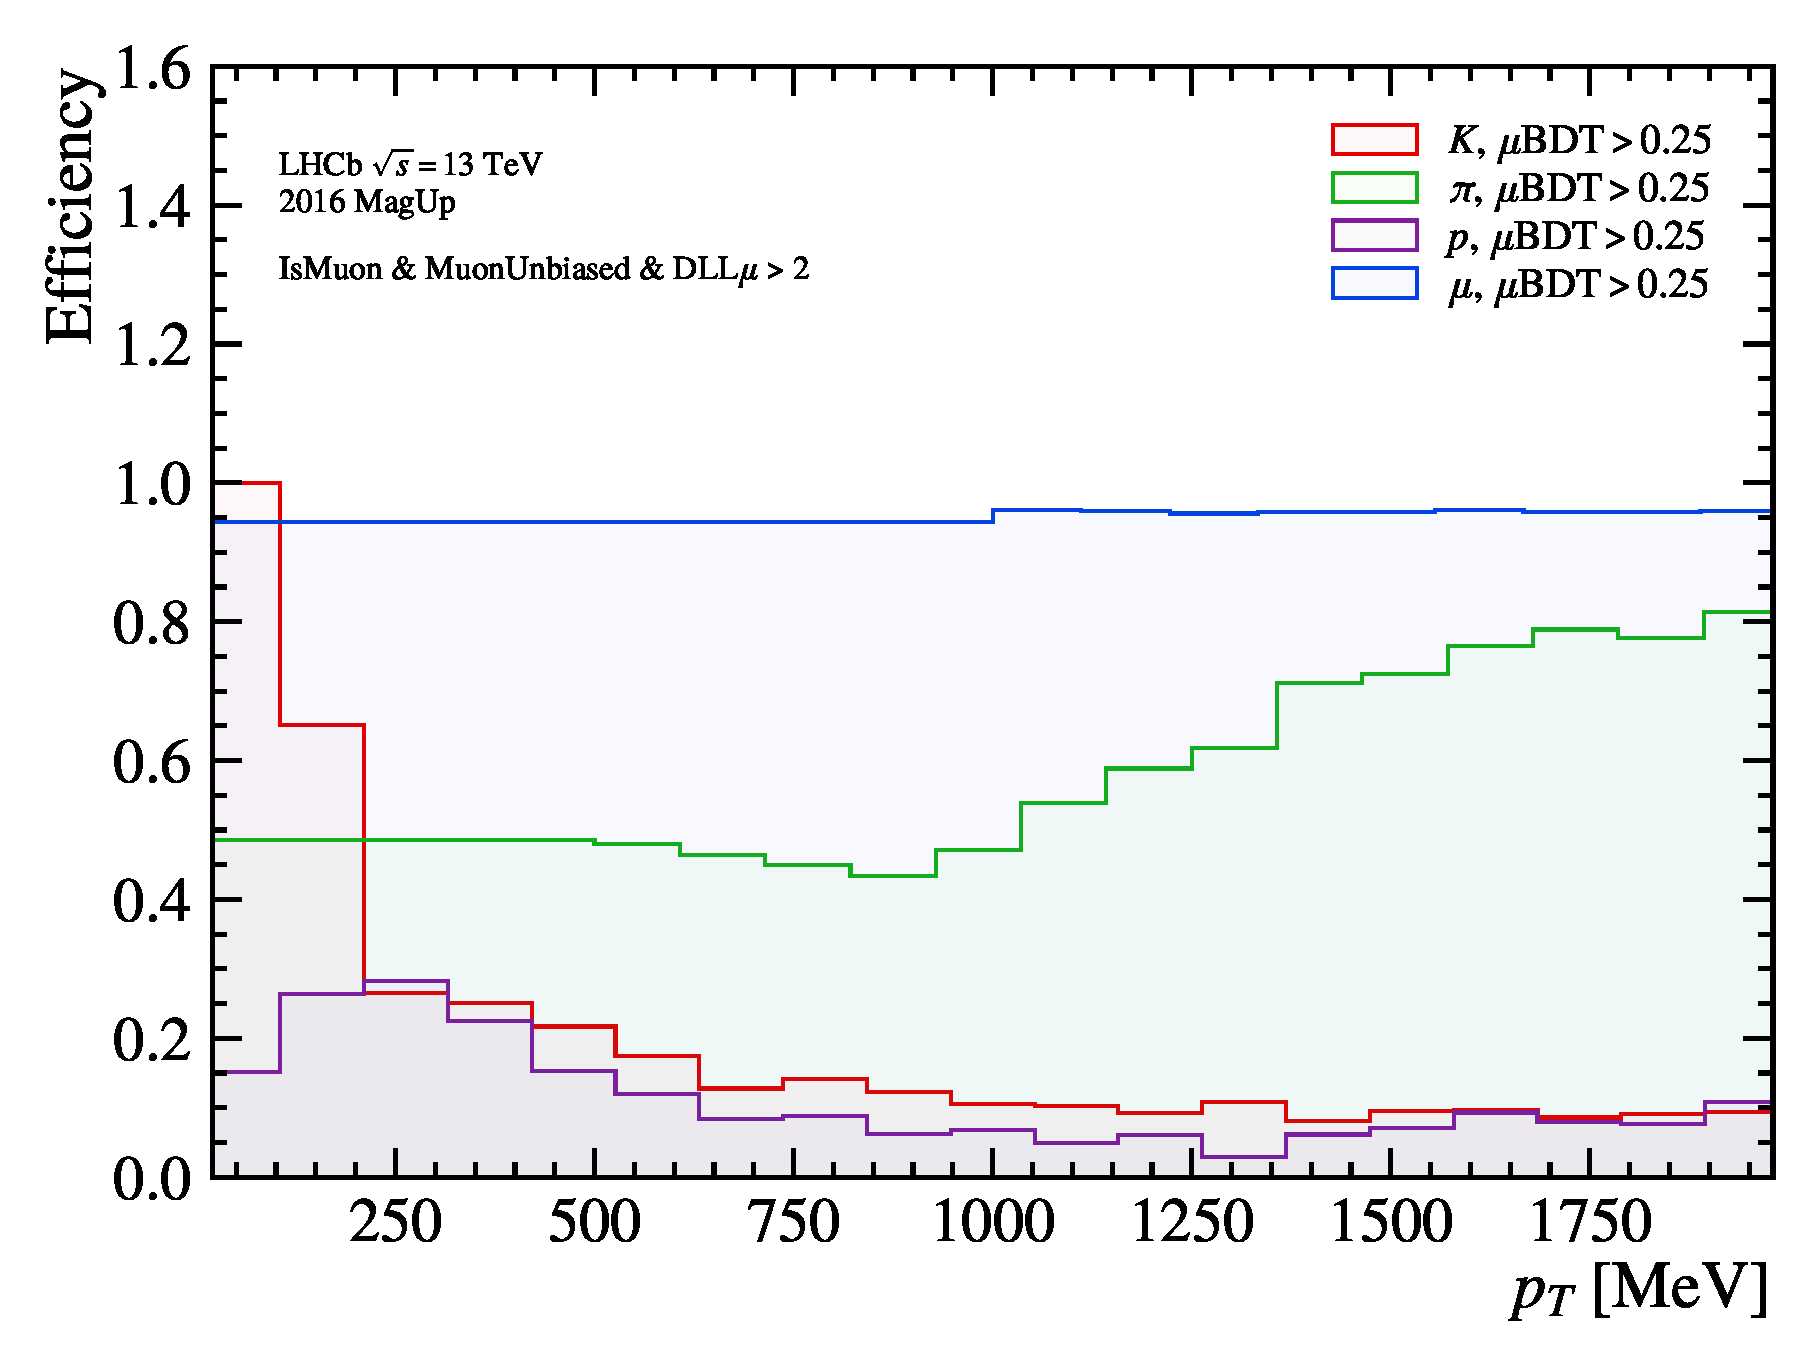
\includegraphics[width=0.45\textwidth]{./figs-selection/eff_Brunel_PT_up_pidcalib_ubdt_eff.pdf}
    \hspace{1em}
    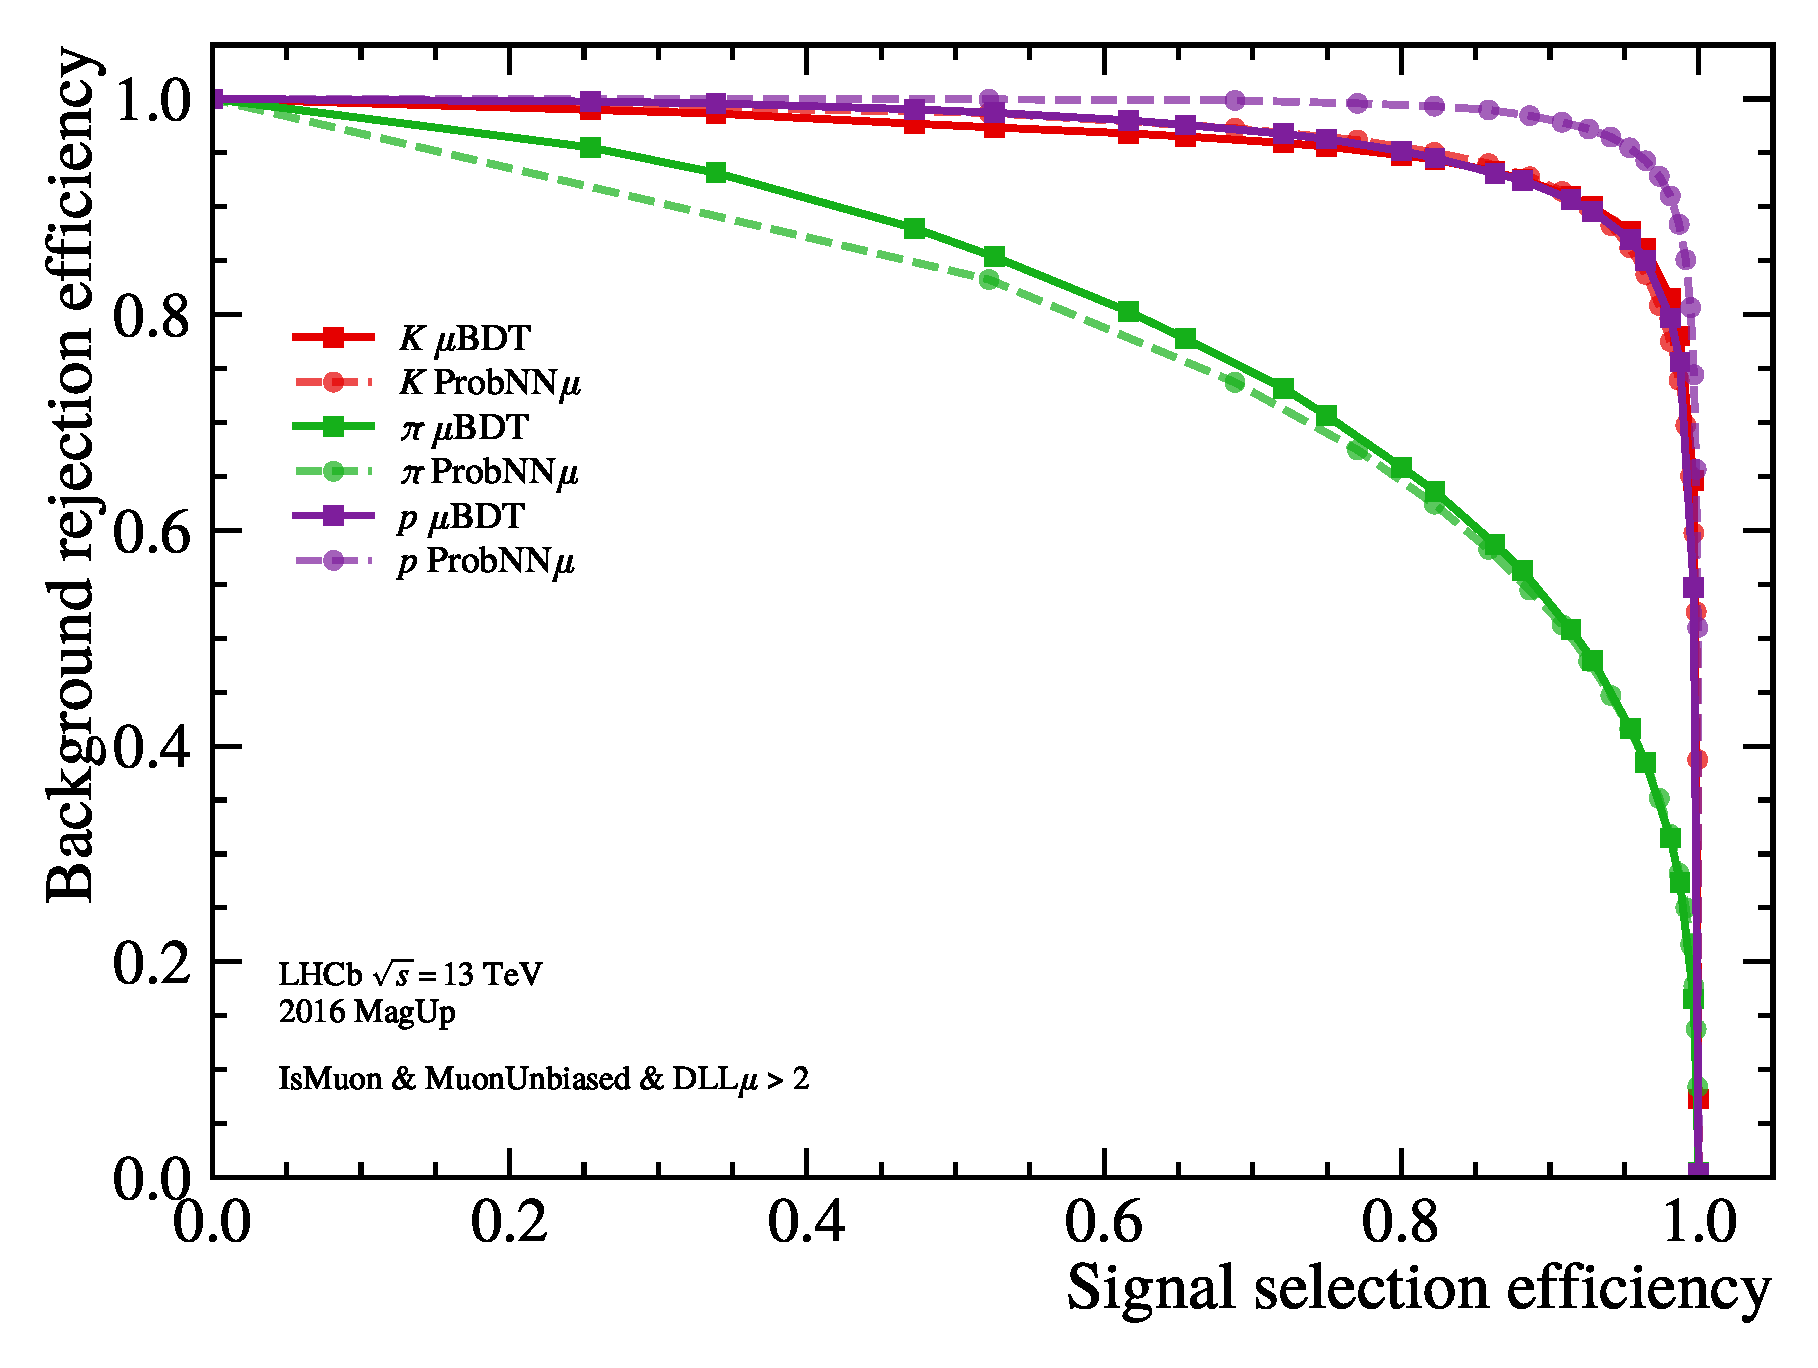
\includegraphics[width=0.45\textwidth]{./figs-selection/rej_v_eff_unbiased_Brunel_PT.pdf}

    \caption{
        Preliminary \UBDT study.
        Left: \UBDT \muon selection efficiency is flat in \pt, with
        global cut \isMuon \& $\text{\PID{\muon}}\! > 2$,
        and $\UBDT > 0.25$.
        Right: with the same global cut, \UBDT is more effective in rejecting
        \pion than LHCb official \ProbNN{\muon}.
        The \kaon rejection efficiencies are similar between the two;
        the $p$ rejection efficiency is lower for \UBDT, but the absolute
        rejection efficiency is high enough.
    }
    \label{fig:ubdt-eff}
\end{figure}



% CHANGES:
% chapter 2: divide into sub-sections (maybe)
%   introduce D**, DDX, background, comb. misID
%     one for D**, one for D** heavy
%   followed by introduction of skims
%  iso: signal sample; ctrl: control samples
%
% chapter 5:
%   5.2, define ghost and cocktail
%   all tracks -> long tracks, find the PT requirement
%   remove the 'likely due to ' part in 5.5.2
%   'refit a vertex' -> ?
%   5.5.2 'improved': forget about saving and ntuple stuff.
%
% chapter 6:
%   TOS and TIS in main text.
%
% chapter 9:
%   explain DiF more


% This table is based on the output of:
%   ./size_mc_samples.py -m detail -i 12573012 11574021 12773410
\begin{landscape}
\begin{table}[p]
    \caption{
        List of MC sample used in this analysis.
        Numbers are event on disk, not total simulated numbers.
    }
    \label{tab:mc-d0-dst}
    \centering\scriptsize
    \begin{longtable}{c|c|c|c|c|r|r|r|r}
        \toprule
        {\bf Group} &
        {\bf MC ID} &
        {\bf Decay mode} &
        {\bf Channels}  &
        {\bf Cocktail}  &
        {\bf\centering \makecell{2016 Sim09j \\ FullSim}} &
        {\bf\centering \makecell{2016 Sim09k \\ tracker-only}} &
        {\bf\centering \makecell{2017 Sim09k \\ tracker-only}} &
        {\bf\centering \makecell{2018 Sim09k \\ tracker-only}} \\
        \midrule
        \endhead
        norm.        & 12573012
                     & $\Bm \rightarrow \Dz \mun \neumb$
                     & \Dz & no
                     %%%%
                     & 3,564,053
                     & 45,564,529
                     & 47,965,869
                     & 64,386,408
                     \\
                     %%%%
                     & 11574021
                     & $\Bzb \rightarrow \Dstarp \mun \neumb$
                     & both & no
                     %%%%
                     & 3,012,029
                     & 85,470,057
                     & 81,075,745
                     & 103,168,826
                     \\
                     %%%%
                     & 12773410
                     & $\Bm \rightarrow \Dstarz \mun \neumb$
                     & \Dz & no
                     %%%%
                     & 4,003,029
                     & 129,200,391
                     & 134,602,735
                     & 169,664,396
                     \\
                     %%%%
        \midrule
        sig.         & 12573001
                     & $\Bm \rightarrow \Dz \taum \neutb$
                     & \Dz & no
                     %%%%
                     & 233,966
                     & 4,152,856
                     & 3,405,213
                     & 4,317,050
                     \\
                     %%%%
                     & 11574011
                     & $\Bzb \rightarrow \Dstarp \taum \neutb$
                     & both & no
                     %%%%
                     & 593,350
                     & 17,217,664
                     & 18,008,069
                     & 25,341,935
                     \\
                     %%%%
                     & 12773400
                     & $\Bm \rightarrow \Dstarz \mun \neumb$
                     & \Dz & no
                     %%%%
                     & 528,616
                     & 9,813,636
                     & 10,289,156
                     & 15,091,483
                     \\
                     %%%%
        \midrule
        $D^{**}$     & 11874430
                     & $\Bzb \rightarrow \D^{**+} \mun \neumb$
                     & both & $D_1^+,D_1^{'+}, D_2^{*+}, D_0^{*+}$
                     %%%%
                     & 2,865,898
                     & 46,653,556
                     & 45,469,066
                     & 58,082,278
                     \\
                     %%%%
                     & 11874440
                     & $\Bzb \rightarrow \D^{**+} \taum \neutb$
                     & both & $D_1^+,D_1^{'+}, D_2^{*+}, D_0^{*+}$
                     %%%%
                     & 35,322
                     & 375,581
                     & 519,245
                     & 561,800
                     \\
                     %%%%
                     & 12873450
                     & $\Bm \rightarrow \D^{**0} \mun \neumb$
                     & both & $D_1^0,D_1^{'0}, D_2^{*0}, D_0^{*0}$
                     %%%%
                     & 2,333,268
                     & 37,417,148
                     & 117,729,837
                     & 48,051,754
                     \\
                     %%%%
                     & 12873460
                     & $\Bm \rightarrow \D^{**0} \taum \neutb$
                     & both & $D_1^0,D_1^{'0}, D_2^{*0}, D_0^{*0}$
                     %%%%
                     & 112,138
                     & 618,529
                     & 598,526
                     & 744,330
                     \\
                     %%%%
        \midrule
        $D^{**}_H$   & 12675011
                     & $\Bm \rightarrow \D^{**0}_H (\rightarrow \Dz\pi\pi) \mun \neumb$
                     & \Dz & \cite{LHCb-ANA-2020-056}
                     %%%%
                     & 419,829
                     & 6,204,217
                     & 7,215,251
                     & 8,573,968
                     \\
                     %%%%
                     & 11674401
                     & $\Bzb \rightarrow \D^{**+}_H (\rightarrow \Dz\pi\pi) \mun \neumb$
                     & \Dz & \cite{LHCb-ANA-2020-056}
                     %%%%
                     & 353,015
                     & 6,997,221
                     & 6,746,518
                     & 12,956,078
                     \\
                     %%%%
                     & 12675402
                     & $\Bm \rightarrow \D^{**0}_H (\rightarrow \Dstarp\pi\pi) \mun \neumb$
                     & both & \cite{LHCb-ANA-2020-056}
                     %%%%
                     & 294,872
                     & 5,560,586
                     & 4,739,776
                     & 6,162,695
                     \\
                     %%%%
                     & 11676012
                     & $\Bzb \rightarrow \D^{**+}_H (\rightarrow \Dstarp\pi\pi) \mun \neumb$
                     & both & \cite{LHCb-ANA-2020-056}
                     %%%%
                     & 290,791
                     & 4,824,507
                     & 4,834,264
                     & 8,353,204
                     \\
                     %%%%
                     & 12875440
                     & $\Bm \rightarrow \D^{**0}_H (\rightarrow \Dstarz\pi\pi) \mun \neumb$
                     & \Dz & \cite{LHCb-ANA-2020-056}
                     %%%%
                     & 450,907
                     & 7,840,307
                     & 7,983,973
                     & 10,039,996
                     \\
                     %%%%
        \midrule
        $D^{**}_s$   & 13874020
                     & $\Bsb \rightarrow \D^{**+}_s (\rightarrow \Dz\Kp) \mun \neumb$
                     & \Dz & no
                     %%%%
                     & 259,166
                     & 1,654,215
                     & 1,732,571
                     & 2,214,625
                     \\
                     %%%%
                     & 13674000
                     & $\Bsb \rightarrow \D^{**+} \mun \neumb$
                     & \Dstar & $D_{s1}^{'+}, D_{s2}^{*+}$
                     %%%%
                     & 142,549
                     & 1,498,067
                     & 1,531,966
                     & 2,070,074
                     \\
                     %%%%
        \midrule
        $DDX$        & 11894600
                     & $\Bzb \rightarrow \Dz X_c (\rightarrow X' \mump \neumb) X$
                     & \Dz & \cite{LHCb-ANA-2020-056}
                     %%%%
                     & 1,062,375
                     & 36,888,835
                     & 37,826,396
                     & 49,768,186
                     \\
                     %%%%
                     & 12893600
                     & $\Bm \rightarrow \Dz X_c (\rightarrow X' \mump \neumb) X$
                     & \Dz & \cite{LHCb-ANA-2020-056}
                     %%%%
                     & 1,196,059
                     & 21,854,863
                     & 22,577,692
                     & 28,900,392
                     \\
                     %%%%
                     & 11894200
                     & $\Bzb \rightarrow \Dz D_s^- (\rightarrow X' \taum \neutb) X$
                     & \Dz & \cite{LHCb-ANA-2020-056}
                     %%%%
                     & 84,533
                     & 1,231,353
                     & 1,145,771
                     & 1,367,357
                     \\
                     %%%%
                     & 12893610
                     & $\Bm \rightarrow \Dz D_s^- (\rightarrow X' \taum \neutb) X$
                     & \Dz & \cite{LHCb-ANA-2020-056}
                     %%%%
                     & 255,725
                     & 2,818,348
                     & 2,625,208
                     & 4,834,213
                     \\
                     %%%%
                     %%%%
                     & 11894610
                     & $\Bzb \rightarrow \Dstarpm X_c (\rightarrow X' \mump \neumb) X$
                     & \Dstar & \cite{LHCb-ANA-2020-056}
                     %%%%
                     & 1,188,596
                     & 16,188,308
                     & 13,480,119
                     & 16,837,410
                     \\
                     %%%%
                     & 12895400
                     & $\Bm \rightarrow \Dstarpm X_c (\rightarrow X' \mump \neumb) X$
                     & \Dstar & \cite{LHCb-ANA-2020-056}
                     %%%%
                     & 365,215
                     & 7,000,178
                     & 7,459,109
                     & 6,798,676
                     \\
                     %%%%
                     & 11894210
                     & $\Bzb \rightarrow \Dstarp D_s^- (\rightarrow X' \taum \neutb) X$
                     & \Dstar & \cite{LHCb-ANA-2020-056}
                     %%%%
                     & 113,422
                     & 1,678,170
                     & 1,283,823
                     & 1,631,217
                     \\
                     %%%%
                     & 12895000
                     & $\Bm \rightarrow \Dstarp D_s^- (\rightarrow X' \taum \neutb) X$
                     & \Dstar & \cite{LHCb-ANA-2020-056}
                     %%%%
                     & 117,696
                     & 899,320
                     & 1,555,844
                     & 1,282,503
                     \\
                     %%%%
        \bottomrule
    \end{longtable}
\end{table}
\end{landscape}



%%%%%%%%%%%%%%
% appendices %
%%%%%%%%%%%%%%
\titleformat{\chapter}{\normalfont\large}{Appendix \thechapter:}{1em}{}

% \include{AppendixA}


%%%%%%%%%%%%%%%%
% bibliography %
%%%%%%%%%%%%%%%%
\normalsize \singlespacing

\addcontentsline{toc}{chapter}{Bibliography}
\printbibliography


\end{document}
